% Options for packages loaded elsewhere
% Options for packages loaded elsewhere
\PassOptionsToPackage{unicode}{hyperref}
\PassOptionsToPackage{hyphens}{url}
%
\documentclass[
  ignorenonframetext,
  aspectratio=169,
  spanish,
]{beamer}
\newif\ifbibliography
\usepackage{pgfpages}
\setbeamertemplate{caption}[numbered]
\setbeamertemplate{caption label separator}{: }
\setbeamercolor{caption name}{fg=normal text.fg}
\beamertemplatenavigationsymbolshorizontal
% remove section numbering
\setbeamertemplate{part page}{
  \centering
  \begin{beamercolorbox}[sep=16pt,center]{part title}
    \usebeamerfont{part title}\insertpart\par
  \end{beamercolorbox}
}
\setbeamertemplate{section page}{
  \centering
  \begin{beamercolorbox}[sep=12pt,center]{section title}
    \usebeamerfont{section title}\insertsection\par
  \end{beamercolorbox}
}
\setbeamertemplate{subsection page}{
  \centering
  \begin{beamercolorbox}[sep=8pt,center]{subsection title}
    \usebeamerfont{subsection title}\insertsubsection\par
  \end{beamercolorbox}
}
% Prevent slide breaks in the middle of a paragraph
\widowpenalties 1 10000
\raggedbottom
\AtBeginPart{
  \frame{\partpage}
}
\AtBeginSection{
  \ifbibliography
  \else
    \frame{\sectionpage}
  \fi
}
\AtBeginSubsection{
  \frame{\subsectionpage}
}
\usepackage{iftex}
\ifPDFTeX
  \usepackage[T1]{fontenc}
  \usepackage[utf8]{inputenc}
  \usepackage{textcomp} % provide euro and other symbols
\else % if luatex or xetex
  \usepackage{unicode-math} % this also loads fontspec
  \defaultfontfeatures{Scale=MatchLowercase}
  \defaultfontfeatures[\rmfamily]{Ligatures=TeX,Scale=1}
\fi
\usepackage{lmodern}

\usetheme[]{default}
\usefonttheme[]{default}
\ifPDFTeX\else
  % xetex/luatex font selection
\fi
% Use upquote if available, for straight quotes in verbatim environments
\IfFileExists{upquote.sty}{\usepackage{upquote}}{}
\IfFileExists{microtype.sty}{% use microtype if available
  \usepackage[]{microtype}
  \UseMicrotypeSet[protrusion]{basicmath} % disable protrusion for tt fonts
}{}
\makeatletter
\@ifundefined{KOMAClassName}{% if non-KOMA class
  \IfFileExists{parskip.sty}{%
    \usepackage{parskip}
  }{% else
    \setlength{\parindent}{0pt}
    \setlength{\parskip}{6pt plus 2pt minus 1pt}}
}{% if KOMA class
  \KOMAoptions{parskip=half}}
\makeatother

\usepackage{color}
\usepackage{fancyvrb}
\newcommand{\VerbBar}{|}
\newcommand{\VERB}{\Verb[commandchars=\\\{\}]}
\DefineVerbatimEnvironment{Highlighting}{Verbatim}{commandchars=\\\{\}}
% Add ',fontsize=\small' for more characters per line
\usepackage{framed}
\definecolor{shadecolor}{RGB}{241,243,245}
\newenvironment{Shaded}{\begin{snugshade}}{\end{snugshade}}
\newcommand{\AlertTok}[1]{\textcolor[rgb]{0.68,0.00,0.00}{#1}}
\newcommand{\AnnotationTok}[1]{\textcolor[rgb]{0.37,0.37,0.37}{#1}}
\newcommand{\AttributeTok}[1]{\textcolor[rgb]{0.40,0.45,0.13}{#1}}
\newcommand{\BaseNTok}[1]{\textcolor[rgb]{0.68,0.00,0.00}{#1}}
\newcommand{\BuiltInTok}[1]{\textcolor[rgb]{0.00,0.23,0.31}{#1}}
\newcommand{\CharTok}[1]{\textcolor[rgb]{0.13,0.47,0.30}{#1}}
\newcommand{\CommentTok}[1]{\textcolor[rgb]{0.37,0.37,0.37}{#1}}
\newcommand{\CommentVarTok}[1]{\textcolor[rgb]{0.37,0.37,0.37}{\textit{#1}}}
\newcommand{\ConstantTok}[1]{\textcolor[rgb]{0.56,0.35,0.01}{#1}}
\newcommand{\ControlFlowTok}[1]{\textcolor[rgb]{0.00,0.23,0.31}{\textbf{#1}}}
\newcommand{\DataTypeTok}[1]{\textcolor[rgb]{0.68,0.00,0.00}{#1}}
\newcommand{\DecValTok}[1]{\textcolor[rgb]{0.68,0.00,0.00}{#1}}
\newcommand{\DocumentationTok}[1]{\textcolor[rgb]{0.37,0.37,0.37}{\textit{#1}}}
\newcommand{\ErrorTok}[1]{\textcolor[rgb]{0.68,0.00,0.00}{#1}}
\newcommand{\ExtensionTok}[1]{\textcolor[rgb]{0.00,0.23,0.31}{#1}}
\newcommand{\FloatTok}[1]{\textcolor[rgb]{0.68,0.00,0.00}{#1}}
\newcommand{\FunctionTok}[1]{\textcolor[rgb]{0.28,0.35,0.67}{#1}}
\newcommand{\ImportTok}[1]{\textcolor[rgb]{0.00,0.46,0.62}{#1}}
\newcommand{\InformationTok}[1]{\textcolor[rgb]{0.37,0.37,0.37}{#1}}
\newcommand{\KeywordTok}[1]{\textcolor[rgb]{0.00,0.23,0.31}{\textbf{#1}}}
\newcommand{\NormalTok}[1]{\textcolor[rgb]{0.00,0.23,0.31}{#1}}
\newcommand{\OperatorTok}[1]{\textcolor[rgb]{0.37,0.37,0.37}{#1}}
\newcommand{\OtherTok}[1]{\textcolor[rgb]{0.00,0.23,0.31}{#1}}
\newcommand{\PreprocessorTok}[1]{\textcolor[rgb]{0.68,0.00,0.00}{#1}}
\newcommand{\RegionMarkerTok}[1]{\textcolor[rgb]{0.00,0.23,0.31}{#1}}
\newcommand{\SpecialCharTok}[1]{\textcolor[rgb]{0.37,0.37,0.37}{#1}}
\newcommand{\SpecialStringTok}[1]{\textcolor[rgb]{0.13,0.47,0.30}{#1}}
\newcommand{\StringTok}[1]{\textcolor[rgb]{0.13,0.47,0.30}{#1}}
\newcommand{\VariableTok}[1]{\textcolor[rgb]{0.07,0.07,0.07}{#1}}
\newcommand{\VerbatimStringTok}[1]{\textcolor[rgb]{0.13,0.47,0.30}{#1}}
\newcommand{\WarningTok}[1]{\textcolor[rgb]{0.37,0.37,0.37}{\textit{#1}}}

\usepackage{longtable,booktabs,array}
\usepackage{calc} % for calculating minipage widths
\usepackage{caption}
% Make caption package work with longtable
\makeatletter
\def\fnum@table{\tablename~\thetable}
\makeatother
\usepackage{graphicx}
\makeatletter
\newsavebox\pandoc@box
\newcommand*\pandocbounded[1]{% scales image to fit in text height/width
  \sbox\pandoc@box{#1}%
  \Gscale@div\@tempa{\textheight}{\dimexpr\ht\pandoc@box+\dp\pandoc@box\relax}%
  \Gscale@div\@tempb{\linewidth}{\wd\pandoc@box}%
  \ifdim\@tempb\p@<\@tempa\p@\let\@tempa\@tempb\fi% select the smaller of both
  \ifdim\@tempa\p@<\p@\scalebox{\@tempa}{\usebox\pandoc@box}%
  \else\usebox{\pandoc@box}%
  \fi%
}
% Set default figure placement to htbp
\def\fps@figure{htbp}
\makeatother



\ifLuaTeX
\usepackage[bidi=basic]{babel}
\else
\usepackage[bidi=default]{babel}
\fi
% get rid of language-specific shorthands (see #6817):
\let\LanguageShortHands\languageshorthands
\def\languageshorthands#1{}


\setlength{\emergencystretch}{3em} % prevent overfull lines

\providecommand{\tightlist}{%
  \setlength{\itemsep}{0pt}\setlength{\parskip}{0pt}}



 


\setbeamertemplate{headline}{} % Elimina la cabecera del tema Madrid
\setbeamertemplate{section in head/foot}{} % Limpia la numeración de secciones
\renewcommand{\contentsname}{Índice}
\renewcommand{\refname}{Referencias}
\renewcommand{\figurename}{Figura}
\renewcommand{\tablename}{Tabla}
\logo{%
  \begin{tabular}{c}
    
\includegraphics[height=1.2cm]{EscudoU.png}
  \end{tabular}%
}
% --- CONFIGURACIÓN DE COLORES INSTITUCIONALES ---
\definecolor{UnicorGreen}{HTML}{024426}
\definecolor{UnicorText}{HTML}{F9F9F9}
\definecolor{UnicorWhite}{HTML}{FFFFFF}
\definecolor{UnicorGold}{HTML}{D1B061}

% Aplicación al fondo y texto general
\setbeamercolor{background canvas}{bg=UnicorGreen}
\setbeamercolor{normal text}{fg=UnicorText}

% Aplicación a títulos y cabeceras
%\setbeamercolor{title}{fg=UnicorWhite}
\setbeamercolor{frametitle}{fg=UnicorWhite}
\setbeamercolor{framesubtitle}{fg=UnicorWhite}

% Aplicación a viñetas y estructura
\setbeamercolor{structure}{fg=UnicorWhite}
\setbeamercolor{itemize item}{fg=UnicorWhite}
\setbeamercolor{itemize subitem}{fg=UnicorWhite}
\setbeamercolor{enumerate item}{fg=UnicorWhite}

% Forzar a LaTeX a repintar el texto general al iniciar el documento
\AtBeginDocument{\usebeamercolor[fg]{normal text}}

% Aplicación a hipervínculos
\hypersetup{colorlinks=true, urlcolor=UnicorGold, linkcolor=UnicorWhite}

% --- ACTIVAR ESTILO DE BLOQUES Y SOMBRAS (ESTILO MADRID) ---
\useinnertheme[shadow=true]{rounded}

% --- COLORES DEL RECUADRO DEL TÍTULO PRINCIPAL ---
% Fondo dorado con texto verde
\setbeamercolor{title}{bg=UnicorGold, fg=UnicorGreen}
\setbeamercolor{frametitle}{fg=UnicorWhite} % Mantiene el título de las diapositivas normal
\setbeamercolor{framesubtitle}{fg=UnicorWhite}

% --- COLORES PARA TEOREMAS, DEFINICIONES Y BLOQUES ---
% Título del bloque (Fondo dorado, texto verde)
\setbeamercolor{block title}{bg=UnicorGold, fg=UnicorGreen}
% Cuerpo del bloque (Fondo blanco, texto verde)
\setbeamercolor{block body}{bg=UnicorWhite, fg=UnicorGreen}

\AtBeginDocument{
  \author{%
    \begin{tabular}{c}
      Mario A. Morales Rivera \\
      \footnotesize \texttt{mamorales@correo.unicordoba.edu.co} \\
      \footnotesize Universidad de Córdoba
    \end{tabular}
  }
  \institute{}
}
% --- LIMPIAR DIAPOSITIVAS DE SECCIÓN (ELIMINAR "SECTION X") ---
\setbeamertemplate{section page}{
  \begin{center}
    \begin{beamercolorbox}[sep=12pt,center,rounded=true,shadow=true]{title}
      \usebeamerfont{title}\insertsection\par
    \end{beamercolorbox}
  \end{center}
}
\makeatletter
\@ifpackageloaded{tcolorbox}{}{\usepackage[skins,breakable]{tcolorbox}}
\@ifpackageloaded{fontawesome5}{}{\usepackage{fontawesome5}}
\definecolor{quarto-callout-color}{HTML}{909090}
\definecolor{quarto-callout-note-color}{HTML}{0758E5}
\definecolor{quarto-callout-important-color}{HTML}{CC1914}
\definecolor{quarto-callout-warning-color}{HTML}{EB9113}
\definecolor{quarto-callout-tip-color}{HTML}{00A047}
\definecolor{quarto-callout-caution-color}{HTML}{FC5300}
\definecolor{quarto-callout-color-frame}{HTML}{acacac}
\definecolor{quarto-callout-note-color-frame}{HTML}{4582ec}
\definecolor{quarto-callout-important-color-frame}{HTML}{d9534f}
\definecolor{quarto-callout-warning-color-frame}{HTML}{f0ad4e}
\definecolor{quarto-callout-tip-color-frame}{HTML}{02b875}
\definecolor{quarto-callout-caution-color-frame}{HTML}{fd7e14}
\makeatother
\makeatletter
\@ifpackageloaded{caption}{}{\usepackage{caption}}
\AtBeginDocument{%
\ifdefined\contentsname
  \renewcommand*\contentsname{Tabla de contenidos}
\else
  \newcommand\contentsname{Tabla de contenidos}
\fi
\ifdefined\listfigurename
  \renewcommand*\listfigurename{Listado de Figuras}
\else
  \newcommand\listfigurename{Listado de Figuras}
\fi
\ifdefined\listtablename
  \renewcommand*\listtablename{Listado de Tablas}
\else
  \newcommand\listtablename{Listado de Tablas}
\fi
\ifdefined\figurename
  \renewcommand*\figurename{Figura}
\else
  \newcommand\figurename{Figura}
\fi
\ifdefined\tablename
  \renewcommand*\tablename{Tabla}
\else
  \newcommand\tablename{Tabla}
\fi
}
\@ifpackageloaded{float}{}{\usepackage{float}}
\floatstyle{ruled}
\@ifundefined{c@chapter}{\newfloat{codelisting}{h}{lop}}{\newfloat{codelisting}{h}{lop}[chapter]}
\floatname{codelisting}{Listado}
\newcommand*\listoflistings{\listof{codelisting}{Listado de Listados}}
\makeatother
\makeatletter
\makeatother
\makeatletter
\@ifpackageloaded{caption}{}{\usepackage{caption}}
\@ifpackageloaded{subcaption}{}{\usepackage{subcaption}}
\makeatother

\usepackage{bookmark}
\IfFileExists{xurl.sty}{\usepackage{xurl}}{} % add URL line breaks if available
\urlstyle{same}
\hypersetup{
  pdftitle={Operaciones con vectores},
  pdfauthor={Mario Morales},
  pdflang={es},
  hidelinks,
  pdfcreator={LaTeX via pandoc}}


\title{Operaciones con vectores}
\author{Mario Morales}
\date{}

\begin{document}
\frame{\titlepage}

\renewcommand*\contentsname{Contenido}
\begin{frame}[allowframebreaks]
  \frametitle{Contenido}
  \setcounter{tocdepth}{3}
  \tableofcontents
\end{frame}
\setcounter{tocdepth}{3}
\tableofcontents
}

\section{Operaciones con vectores}\label{operaciones-con-vectores}

\begin{frame}{¿Qué aprenderemos?}
\phantomsection\label{quuxe9-aprenderemos}
\begin{itemize}
\tightlist
\item
  Comprender el concepto de vectorización en R
\item
  Comprender qué son los vectores lógicos y cómo manipularlos.
\item
  Usar la indexación lógica para seleccionar subconjuntos de un vector.
\item
  Ser capaz de utilizar valores infinitos y perdidos.
\end{itemize}
\end{frame}

\begin{frame}[fragile]{Operaciones con vectores}
\phantomsection\label{operaciones-con-vectores-1}
Los vectores son muy útiles porque permiten a R realizar operaciones en
múltiples elementos simultáneamente, con velocidad y eficiencia. Este
comportamiento \texttt{orientado\ a\ vectores}, \texttt{vectorizado} o
\texttt{de\ elementos} es una característica clave del lenguaje.
\end{frame}

\begin{frame}[fragile]{}
\phantomsection\label{section}
\begin{Shaded}
\begin{Highlighting}[]
\DecValTok{1}\SpecialCharTok{:}\DecValTok{5}
\end{Highlighting}
\end{Shaded}

\begin{verbatim}
[1] 1 2 3 4 5
\end{verbatim}

\begin{Shaded}
\begin{Highlighting}[]
\CommentTok{\#class(1:5)}
\CommentTok{\#mode(1:5)}
\DecValTok{6}\SpecialCharTok{:}\DecValTok{10}
\end{Highlighting}
\end{Shaded}

\begin{verbatim}
[1]  6  7  8  9 10
\end{verbatim}

\begin{Shaded}
\begin{Highlighting}[]
\DecValTok{1}\SpecialCharTok{:}\DecValTok{5} \SpecialCharTok{+} \DecValTok{6}\SpecialCharTok{:}\DecValTok{10} \CommentTok{\# vectorizacion  }
\end{Highlighting}
\end{Shaded}

\begin{verbatim}
[1]  7  9 11 13 15
\end{verbatim}
\end{frame}

\begin{frame}[fragile]{Operación Suma}
\phantomsection\label{operaciuxf3n-suma}
La operación suma de dos vectores se hace componente a componente

\begin{Shaded}
\begin{Highlighting}[]
\FunctionTok{c}\NormalTok{(}\DecValTok{1}\NormalTok{, }\DecValTok{3}\NormalTok{, }\DecValTok{6}\NormalTok{, }\DecValTok{10}\NormalTok{, }\DecValTok{15}\NormalTok{) }\SpecialCharTok{+} \FunctionTok{c}\NormalTok{(}\DecValTok{0}\NormalTok{, }\DecValTok{1}\NormalTok{, }\DecValTok{3}\NormalTok{, }\DecValTok{6}\NormalTok{, }\DecValTok{10}\NormalTok{) }
\end{Highlighting}
\end{Shaded}

\begin{verbatim}
[1]  1  4  9 16 25
\end{verbatim}
\end{frame}

\begin{frame}[fragile]{Operación Resta}
\phantomsection\label{operaciuxf3n-resta}
La operación resta de dos vectores se hace componente a componente

\begin{Shaded}
\begin{Highlighting}[]
\FunctionTok{c}\NormalTok{(}\DecValTok{1}\NormalTok{, }\DecValTok{3}\NormalTok{, }\DecValTok{6}\NormalTok{, }\DecValTok{10}\NormalTok{, }\DecValTok{15}\NormalTok{) }\SpecialCharTok{{-}} \FunctionTok{c}\NormalTok{(}\DecValTok{0}\NormalTok{, }\DecValTok{1}\NormalTok{, }\DecValTok{3}\NormalTok{, }\DecValTok{6}\NormalTok{, }\DecValTok{10}\NormalTok{) }
\end{Highlighting}
\end{Shaded}

\begin{verbatim}
[1] 1 2 3 4 5
\end{verbatim}
\end{frame}

\begin{frame}[fragile]{Operación producto}
\phantomsection\label{operaciuxf3n-producto}
La operación producto de dos vectores se hace componente a componente

\begin{Shaded}
\begin{Highlighting}[]
\FunctionTok{c}\NormalTok{(}\DecValTok{1}\NormalTok{, }\DecValTok{3}\NormalTok{, }\DecValTok{6}\NormalTok{, }\DecValTok{10}\NormalTok{, }\DecValTok{15}\NormalTok{) }\SpecialCharTok{*} \FunctionTok{c}\NormalTok{(}\DecValTok{0}\NormalTok{, }\DecValTok{1}\NormalTok{, }\DecValTok{3}\NormalTok{, }\DecValTok{6}\NormalTok{, }\DecValTok{10}\NormalTok{) }
\end{Highlighting}
\end{Shaded}

\begin{verbatim}
[1]   0   3  18  60 150
\end{verbatim}
\end{frame}

\begin{frame}[fragile]{Operación cociente}
\phantomsection\label{operaciuxf3n-cociente}
La operación cociente de dos vectores se hace componente a componente

\begin{Shaded}
\begin{Highlighting}[]
\FunctionTok{c}\NormalTok{(}\DecValTok{1}\NormalTok{, }\DecValTok{3}\NormalTok{, }\DecValTok{6}\NormalTok{, }\DecValTok{10}\NormalTok{, }\DecValTok{15}\NormalTok{) }\SpecialCharTok{/} \FunctionTok{c}\NormalTok{(}\DecValTok{0}\NormalTok{, }\DecValTok{1}\NormalTok{, }\DecValTok{3}\NormalTok{, }\DecValTok{6}\NormalTok{, }\DecValTok{10}\NormalTok{) }
\end{Highlighting}
\end{Shaded}

\begin{verbatim}
[1]      Inf 3.000000 2.000000 1.666667 1.500000
\end{verbatim}
\end{frame}

\begin{frame}[fragile]{Reciclado de valores}
\phantomsection\label{reciclado-de-valores}
Cuando los vectores no tienen la misma longitud, el vector más corto se
replica hasta alcanzar la longitud del más largo. En caso de que la
longitud del más largo no sea un múltiplo de la longitud del más corto
manda un mensaje de advertencia.

\begin{Shaded}
\begin{Highlighting}[]
\FunctionTok{c}\NormalTok{(}\DecValTok{1}\NormalTok{, }\DecValTok{3}\NormalTok{, }\DecValTok{6}\NormalTok{, }\DecValTok{10}\NormalTok{, }\DecValTok{15}\NormalTok{,}\DecValTok{17}\NormalTok{)}\SpecialCharTok{+}\FunctionTok{c}\NormalTok{(}\DecValTok{3}\NormalTok{,}\DecValTok{6}\NormalTok{,}\DecValTok{8}\NormalTok{)}
\end{Highlighting}
\end{Shaded}

\begin{verbatim}
[1]  4  9 14 13 21 25
\end{verbatim}
\end{frame}

\begin{frame}[fragile]{Reciclado de valores (II)}
\phantomsection\label{reciclado-de-valores-ii}
\begin{Shaded}
\begin{Highlighting}[]
\CommentTok{\# mensaje de advertencia }
\FunctionTok{c}\NormalTok{(}\DecValTok{1}\NormalTok{, }\DecValTok{3}\NormalTok{, }\DecValTok{6}\NormalTok{, }\DecValTok{10}\NormalTok{, }\DecValTok{15}\NormalTok{,}\DecValTok{17}\NormalTok{)}\SpecialCharTok{+}\FunctionTok{c}\NormalTok{(}\DecValTok{3}\NormalTok{,}\DecValTok{6}\NormalTok{,}\DecValTok{8}\NormalTok{,}\DecValTok{10}\NormalTok{)  }
\end{Highlighting}
\end{Shaded}

\begin{verbatim}
[1]  4  9 14 20 18 23
\end{verbatim}

\begin{verbatim}
Warning message in c(1, 3, 6, 10, 15, 17) + c(3, 6, 8, 10):
“longitud de objeto mayor no es múltiplo de la longitud de uno menor”
\end{verbatim}
\end{frame}

\begin{frame}[fragile]{Resta}
\phantomsection\label{resta}
\begin{Shaded}
\begin{Highlighting}[]
\NormalTok{foo}\OtherTok{\textless{}{-}}\FunctionTok{c}\NormalTok{(}\DecValTok{1}\NormalTok{, }\DecValTok{3}\NormalTok{, }\DecValTok{6}\NormalTok{, }\DecValTok{10}\NormalTok{, }\DecValTok{15}\NormalTok{,}\DecValTok{17}\NormalTok{)}
\NormalTok{bar}\OtherTok{\textless{}{-}}\FunctionTok{c}\NormalTok{(}\DecValTok{3}\NormalTok{,}\DecValTok{6}\NormalTok{,}\DecValTok{8}\NormalTok{)}
\NormalTok{foo}\SpecialCharTok{{-}}\NormalTok{bar}
\end{Highlighting}
\end{Shaded}

\begin{verbatim}
[1] -2 -3 -2  7  9  9
\end{verbatim}
\end{frame}

\begin{frame}[fragile]{¿Cómo trabaja?}
\phantomsection\label{cuxf3mo-trabaja}
\begin{Shaded}
\begin{Highlighting}[]
\NormalTok{x}\OtherTok{=}\FunctionTok{rep}\NormalTok{(}\SpecialCharTok{{-}}\DecValTok{1}\NormalTok{,}\FunctionTok{length}\NormalTok{(foo)) }
\FunctionTok{plot}\NormalTok{(x,}\DecValTok{1}\SpecialCharTok{:}\FunctionTok{length}\NormalTok{(foo),}\AttributeTok{axes=}\ConstantTok{FALSE}\NormalTok{,}\AttributeTok{ann=}\ConstantTok{FALSE}\NormalTok{,}\AttributeTok{type=}\StringTok{"p"}\NormalTok{,}\AttributeTok{col=}\StringTok{\textquotesingle{}white\textquotesingle{}}\NormalTok{,}\AttributeTok{xlim=}\FunctionTok{c}\NormalTok{(}\SpecialCharTok{{-}}\DecValTok{2}\NormalTok{,}\DecValTok{2}\NormalTok{))}
\FunctionTok{arrows}\NormalTok{(x}\FloatTok{{-}0.5}\NormalTok{,}\FunctionTok{length}\NormalTok{(foo)}\SpecialCharTok{:}\DecValTok{1}\NormalTok{,x}\FloatTok{+0.5}\NormalTok{,}\FunctionTok{length}\NormalTok{(foo)}\SpecialCharTok{:}\DecValTok{1}\NormalTok{,}\AttributeTok{code=}\DecValTok{3}\NormalTok{,}\AttributeTok{angle=}\DecValTok{20}\NormalTok{,}\AttributeTok{length =} \FloatTok{0.15}\NormalTok{)}
\FunctionTok{text}\NormalTok{(x}\FloatTok{{-}0.6}\NormalTok{,}\FunctionTok{length}\NormalTok{(foo)}\SpecialCharTok{:}\DecValTok{1}\NormalTok{,}\AttributeTok{labels=}\NormalTok{foo)}
\FunctionTok{text}\NormalTok{(x}\FloatTok{{-}0.8}\NormalTok{,}\FunctionTok{length}\NormalTok{(foo)}\SpecialCharTok{:}\DecValTok{1}\NormalTok{,}\AttributeTok{labels=}\FunctionTok{paste}\NormalTok{(}\StringTok{\textquotesingle{}[\textquotesingle{}}\NormalTok{,}\DecValTok{1}\SpecialCharTok{:}\FunctionTok{length}\NormalTok{(foo),}\StringTok{\textquotesingle{}]\textquotesingle{}}\NormalTok{,}\AttributeTok{sep=}\StringTok{\textquotesingle{}\textquotesingle{}}\NormalTok{))}
\FunctionTok{text}\NormalTok{(x}\FloatTok{+0.6}\NormalTok{,}\FunctionTok{length}\NormalTok{(foo)}\SpecialCharTok{:}\DecValTok{1}\NormalTok{,}\AttributeTok{labels=}\NormalTok{bar)}
\FunctionTok{text}\NormalTok{(x}\FloatTok{+0.8}\NormalTok{,}\FunctionTok{length}\NormalTok{(foo)}\SpecialCharTok{:}\DecValTok{1}\NormalTok{,}\AttributeTok{labels=}\FunctionTok{paste}\NormalTok{(}\StringTok{\textquotesingle{}[\textquotesingle{}}\NormalTok{,}\DecValTok{1}\SpecialCharTok{:}\FunctionTok{length}\NormalTok{(bar),}\StringTok{\textquotesingle{}]\textquotesingle{}}\NormalTok{,}\AttributeTok{sep=}\StringTok{\textquotesingle{}\textquotesingle{}}\NormalTok{))}
\FunctionTok{text}\NormalTok{(x}\FloatTok{+0.8}\NormalTok{,}\FunctionTok{length}\NormalTok{(foo)}\SpecialCharTok{:}\DecValTok{1}\NormalTok{,}\AttributeTok{labels=}\FunctionTok{paste}\NormalTok{(}\StringTok{\textquotesingle{}[\textquotesingle{}}\NormalTok{,}\DecValTok{1}\SpecialCharTok{:}\FunctionTok{length}\NormalTok{(bar),}\StringTok{\textquotesingle{}]\textquotesingle{}}\NormalTok{,}\AttributeTok{sep=}\StringTok{\textquotesingle{}\textquotesingle{}}\NormalTok{))}
\FunctionTok{mtext}\NormalTok{(}\StringTok{"foo"}\NormalTok{,}\AttributeTok{side=}\DecValTok{3}\NormalTok{, }\AttributeTok{at=}\SpecialCharTok{{-}}\DecValTok{1}\FloatTok{{-}0.8}\NormalTok{)}
\FunctionTok{mtext}\NormalTok{(}\StringTok{"bar"}\NormalTok{,}\AttributeTok{side=}\DecValTok{3}\NormalTok{, }\AttributeTok{at=}\SpecialCharTok{{-}}\DecValTok{1}\FloatTok{+0.8}\NormalTok{)}
\FunctionTok{mtext}\NormalTok{(}\StringTok{"\_"}\NormalTok{,}\AttributeTok{side=}\DecValTok{3}\NormalTok{, }\AttributeTok{at=}\SpecialCharTok{{-}}\DecValTok{1}\NormalTok{)}

\CommentTok{\# cuando la longitud del más corto no es divisor de la long del mas largo}
\NormalTok{x}\OtherTok{=}\FunctionTok{rep}\NormalTok{(}\DecValTok{1}\NormalTok{,}\FunctionTok{length}\NormalTok{(foo))}
\NormalTok{bar}\OtherTok{\textless{}{-}}\FunctionTok{c}\NormalTok{(}\DecValTok{3}\NormalTok{,}\DecValTok{6}\NormalTok{,}\DecValTok{8}\NormalTok{,}\DecValTok{4}\NormalTok{)}

\FunctionTok{arrows}\NormalTok{(x}\FloatTok{{-}0.5}\NormalTok{,}\FunctionTok{length}\NormalTok{(foo)}\SpecialCharTok{:}\DecValTok{1}\NormalTok{,x}\FloatTok{+0.5}\NormalTok{,}\FunctionTok{length}\NormalTok{(foo)}\SpecialCharTok{:}\DecValTok{1}\NormalTok{,}\AttributeTok{code=}\DecValTok{3}\NormalTok{,}\AttributeTok{angle=}\DecValTok{20}\NormalTok{,}\AttributeTok{length =} \FloatTok{0.15}\NormalTok{)}
\FunctionTok{text}\NormalTok{(x}\FloatTok{{-}0.6}\NormalTok{,}\FunctionTok{length}\NormalTok{(foo)}\SpecialCharTok{:}\DecValTok{1}\NormalTok{,}\AttributeTok{labels=}\NormalTok{foo)}
\FunctionTok{text}\NormalTok{(x}\FloatTok{{-}0.8}\NormalTok{,}\FunctionTok{length}\NormalTok{(foo)}\SpecialCharTok{:}\DecValTok{1}\NormalTok{,}\AttributeTok{labels=}\FunctionTok{paste}\NormalTok{(}\StringTok{\textquotesingle{}[\textquotesingle{}}\NormalTok{,}\DecValTok{1}\SpecialCharTok{:}\FunctionTok{length}\NormalTok{(foo),}\StringTok{\textquotesingle{}]\textquotesingle{}}\NormalTok{,}\AttributeTok{sep=}\StringTok{\textquotesingle{}\textquotesingle{}}\NormalTok{))}
\FunctionTok{text}\NormalTok{(x}\FloatTok{+0.6}\NormalTok{,}\FunctionTok{length}\NormalTok{(foo)}\SpecialCharTok{:}\DecValTok{1}\NormalTok{,}\AttributeTok{labels=}\NormalTok{bar)}
\FunctionTok{text}\NormalTok{(x}\FloatTok{+0.8}\NormalTok{,}\FunctionTok{length}\NormalTok{(foo)}\SpecialCharTok{:}\DecValTok{1}\NormalTok{,}\AttributeTok{labels=}\FunctionTok{paste}\NormalTok{(}\StringTok{\textquotesingle{}[\textquotesingle{}}\NormalTok{,}\DecValTok{1}\SpecialCharTok{:}\FunctionTok{length}\NormalTok{(bar),}\StringTok{\textquotesingle{}]\textquotesingle{}}\NormalTok{,}\AttributeTok{sep=}\StringTok{\textquotesingle{}\textquotesingle{}}\NormalTok{))}
\FunctionTok{text}\NormalTok{(x}\FloatTok{+0.8}\NormalTok{,}\FunctionTok{length}\NormalTok{(foo)}\SpecialCharTok{:}\DecValTok{1}\NormalTok{,}\AttributeTok{labels=}\FunctionTok{paste}\NormalTok{(}\StringTok{\textquotesingle{}[\textquotesingle{}}\NormalTok{,}\DecValTok{1}\SpecialCharTok{:}\FunctionTok{length}\NormalTok{(bar),}\StringTok{\textquotesingle{}]\textquotesingle{}}\NormalTok{,}\AttributeTok{sep=}\StringTok{\textquotesingle{}\textquotesingle{}}\NormalTok{))}
\FunctionTok{mtext}\NormalTok{(}\StringTok{"foo"}\NormalTok{,}\AttributeTok{side=}\DecValTok{3}\NormalTok{, }\AttributeTok{at=}\DecValTok{1}\FloatTok{{-}0.8}\NormalTok{)}
\FunctionTok{mtext}\NormalTok{(}\StringTok{"bar"}\NormalTok{,}\AttributeTok{side=}\DecValTok{3}\NormalTok{, }\AttributeTok{at=}\DecValTok{1}\FloatTok{+0.8}\NormalTok{)}
\FunctionTok{mtext}\NormalTok{(}\StringTok{"\_"}\NormalTok{,}\AttributeTok{side=}\DecValTok{3}\NormalTok{, }\AttributeTok{at=}\DecValTok{1}\NormalTok{)}
\end{Highlighting}
\end{Shaded}

\pandocbounded{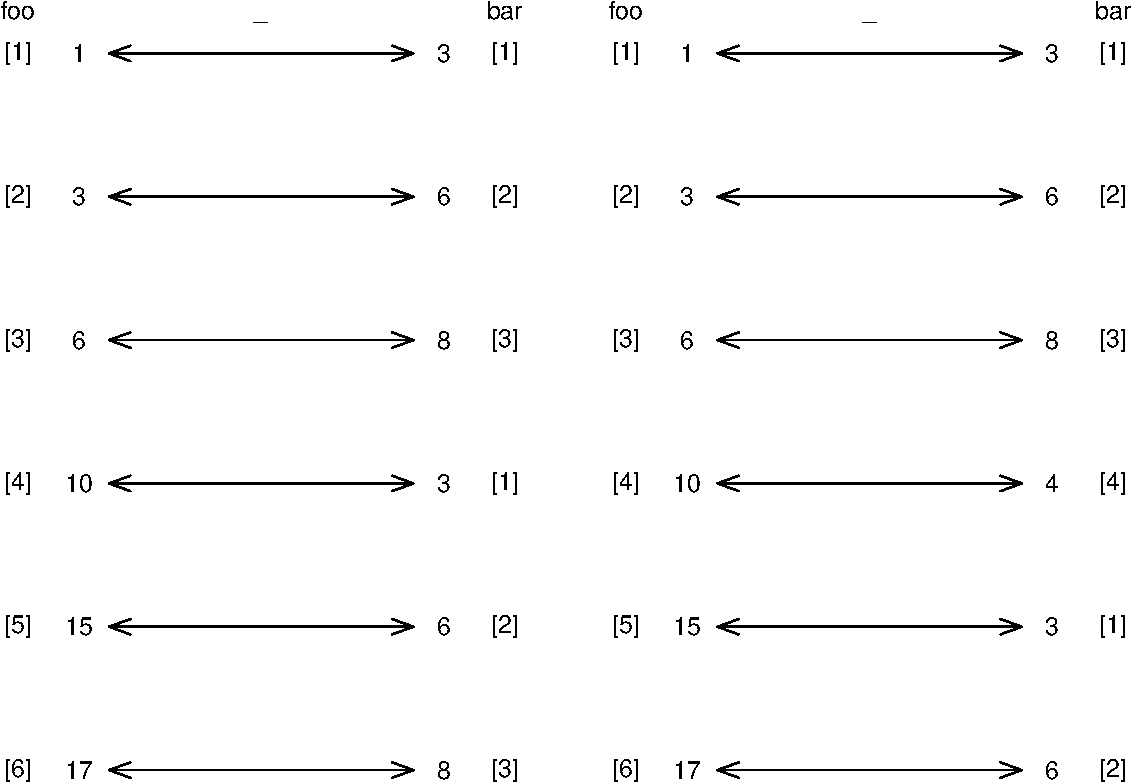
\includegraphics[keepaspectratio]{Clase2OperConVectores2026-1_files/figure-beamer/unnamed-chunk-9-1.pdf}}
\end{frame}

\begin{frame}{Vectorización}
\phantomsection\label{vectorizaciuxf3n}
\begin{itemize}
\tightlist
\item
  \textbf{En las operaciones anteriores se ha usado el concepto de
  \emph{vectorización}}, el cual tiene varios significados en R, el más
  común de los cuales es que
\end{itemize}

\begin{tcolorbox}[enhanced jigsaw, leftrule=.75mm, opacitybacktitle=0.6, opacityback=0, coltitle=black, breakable, colbacktitle=quarto-callout-important-color!10!white, colback=white, titlerule=0mm, bottomrule=.15mm, left=2mm, bottomtitle=1mm, colframe=quarto-callout-important-color-frame, toptitle=1mm, toprule=.15mm, title=\textcolor{quarto-callout-important-color}{\faExclamation}\hspace{0.5em}{Importante}, arc=.35mm, rightrule=.15mm]

Un operador o una función actuará sobre cada elemento de un vector sin
la necesidad de que usted escriba un bucle.

\end{tcolorbox}
\end{frame}

\begin{frame}[fragile]{Vectorización: segundo significado}
\phantomsection\label{vectorizaciuxf3n-segundo-significado}
\begin{itemize}
\tightlist
\item
  Un segundo significado de \emph{vectorización} es cuando una función
  toma un vector como entrada y calcula una estadística de resumen.
\end{itemize}

\begin{Shaded}
\begin{Highlighting}[]
\CommentTok{\# primer concepto de vectorización}
\NormalTok{x}\OtherTok{=}\FunctionTok{c}\NormalTok{(}\DecValTok{3}\NormalTok{,}\DecValTok{5}\NormalTok{,}\DecValTok{1}\NormalTok{,}\DecValTok{7}\NormalTok{,}\DecValTok{4}\NormalTok{) }
\CommentTok{\# raiz usando vectorizacion}
\FunctionTok{sqrt}\NormalTok{(x)}
\end{Highlighting}
\end{Shaded}

\begin{verbatim}
[1] 1.732051 2.236068 1.000000 2.645751 2.000000
\end{verbatim}

\begin{Shaded}
\begin{Highlighting}[]
\FunctionTok{sqrt}\NormalTok{(}\FunctionTok{c}\NormalTok{(}\DecValTok{4}\NormalTok{,}\DecValTok{9}\NormalTok{,}\DecValTok{16}\NormalTok{,}\DecValTok{1}\NormalTok{)) }
\end{Highlighting}
\end{Shaded}

\begin{verbatim}
[1] 2 3 4 1
\end{verbatim}
\end{frame}

\begin{frame}[fragile]{Sin Vectorización (no recomendado)}
\phantomsection\label{sin-vectorizaciuxf3n-no-recomendado}
\begin{Shaded}
\begin{Highlighting}[]
\CommentTok{\# raiz usando un bucle for }
\CommentTok{\# no recomendado}
\ControlFlowTok{for}\NormalTok{(i }\ControlFlowTok{in}\NormalTok{ x)\{}
\FunctionTok{print}\NormalTok{(}\FunctionTok{sqrt}\NormalTok{(i))}
\NormalTok{\}}
\end{Highlighting}
\end{Shaded}

\begin{verbatim}
[1] 1.732051
[1] 2.236068
[1] 1
[1] 2.645751
[1] 2
\end{verbatim}
\end{frame}

\begin{frame}[fragile]{Segundo concepto de vectorizacion}
\phantomsection\label{segundo-concepto-de-vectorizacion}
\begin{Shaded}
\begin{Highlighting}[]
\CommentTok{\# segundo concepto de vectorizacion }
\CommentTok{\# la función se aplica sobre un vector}
\FunctionTok{sum}\NormalTok{(}\DecValTok{1}\SpecialCharTok{:}\DecValTok{5}\NormalTok{)  }
\end{Highlighting}
\end{Shaded}

\begin{verbatim}
[1] 15
\end{verbatim}

\begin{Shaded}
\begin{Highlighting}[]
\FunctionTok{sum}\NormalTok{(x)}
\end{Highlighting}
\end{Shaded}

\begin{verbatim}
[1] 20
\end{verbatim}

\begin{Shaded}
\begin{Highlighting}[]
\FunctionTok{median}\NormalTok{(}\DecValTok{1}\SpecialCharTok{:}\DecValTok{5}\NormalTok{) }
\end{Highlighting}
\end{Shaded}

\begin{verbatim}
[1] 3
\end{verbatim}

\begin{Shaded}
\begin{Highlighting}[]
\FunctionTok{median}\NormalTok{(x)}
\end{Highlighting}
\end{Shaded}

\begin{verbatim}
[1] 4
\end{verbatim}
\end{frame}

\begin{frame}[fragile]{Ejemplos de vectorización}
\phantomsection\label{ejemplos-de-vectorizaciuxf3n}
Todos los operadores aritméticos en R están vectorizados. Los siguientes
ejemplos demuestran la resta, la multiplicación, la exponenciación y dos
tipos de división, así como el residuo de la división:

\begin{Shaded}
\begin{Highlighting}[]
\FunctionTok{c}\NormalTok{(}\DecValTok{2}\NormalTok{, }\DecValTok{3}\NormalTok{, }\DecValTok{5}\NormalTok{, }\DecValTok{7}\NormalTok{, }\DecValTok{11}\NormalTok{, }\DecValTok{13}\NormalTok{) }\SpecialCharTok{{-}} \DecValTok{2}  \CommentTok{\#subtración  }
\end{Highlighting}
\end{Shaded}

\begin{verbatim}
[1]  0  1  3  5  9 11
\end{verbatim}

\begin{Shaded}
\begin{Highlighting}[]
\SpecialCharTok{{-}}\DecValTok{2}\SpecialCharTok{:}\DecValTok{2} \SpecialCharTok{*} \SpecialCharTok{{-}}\DecValTok{2}\SpecialCharTok{:}\DecValTok{2} \CommentTok{\#multiplicación }
\end{Highlighting}
\end{Shaded}

\begin{verbatim}
[1] 4 1 0 1 4
\end{verbatim}

\begin{Shaded}
\begin{Highlighting}[]
\DecValTok{1}\SpecialCharTok{:}\DecValTok{10} \SpecialCharTok{/} \DecValTok{3}  \DocumentationTok{\#\# división usual (de punto flotante)}
\end{Highlighting}
\end{Shaded}

\begin{verbatim}
 [1] 0.3333333 0.6666667 1.0000000 1.3333333 1.6666667 2.0000000 2.3333333
 [8] 2.6666667 3.0000000 3.3333333
\end{verbatim}

\begin{Shaded}
\begin{Highlighting}[]
\DecValTok{1}\SpecialCharTok{:}\DecValTok{10} \SpecialCharTok{\%/\%} \DecValTok{3} \DocumentationTok{\#\# división entera }
\end{Highlighting}
\end{Shaded}

\begin{verbatim}
 [1] 0 0 1 1 1 2 2 2 3 3
\end{verbatim}

\begin{Shaded}
\begin{Highlighting}[]
\DecValTok{1}\SpecialCharTok{:}\DecValTok{10} \SpecialCharTok{\%\%} \DecValTok{3} \DocumentationTok{\#\# residuo de la división}
\end{Highlighting}
\end{Shaded}

\begin{verbatim}
 [1] 1 2 0 1 2 0 1 2 0 1
\end{verbatim}
\end{frame}

\begin{frame}[fragile]{Ejemplo de aplicación}
\phantomsection\label{ejemplo-de-aplicaciuxf3n}
\begin{tcolorbox}[enhanced jigsaw, leftrule=.75mm, opacitybacktitle=0.6, opacityback=0, coltitle=black, breakable, colbacktitle=quarto-callout-important-color!10!white, colback=white, titlerule=0mm, bottomrule=.15mm, left=2mm, bottomtitle=1mm, colframe=quarto-callout-important-color-frame, toptitle=1mm, toprule=.15mm, title=\textcolor{quarto-callout-important-color}{\faExclamation}\hspace{0.5em}{Importante}, arc=.35mm, rightrule=.15mm]

¿Cuántos números del 1 al 10 son divisibles por 3?

\end{tcolorbox}

\begin{Shaded}
\begin{Highlighting}[]
\DecValTok{1}\SpecialCharTok{:}\DecValTok{10} \SpecialCharTok{\%\%} \DecValTok{3} 
\end{Highlighting}
\end{Shaded}

\begin{verbatim}
 [1] 1 2 0 1 2 0 1 2 0 1
\end{verbatim}

\begin{Shaded}
\begin{Highlighting}[]
\DecValTok{1}\SpecialCharTok{:}\DecValTok{10} \SpecialCharTok{\%\%} \DecValTok{3} \SpecialCharTok{==} \DecValTok{0} 
\end{Highlighting}
\end{Shaded}

\begin{verbatim}
 [1] FALSE FALSE  TRUE FALSE FALSE  TRUE FALSE FALSE  TRUE FALSE
\end{verbatim}

\begin{Shaded}
\begin{Highlighting}[]
\FunctionTok{sum}\NormalTok{(}\DecValTok{1}\SpecialCharTok{:}\DecValTok{10} \SpecialCharTok{\%\%} \DecValTok{3} \SpecialCharTok{==}\DecValTok{0}\NormalTok{ )  }
\end{Highlighting}
\end{Shaded}

\begin{verbatim}
[1] 3
\end{verbatim}

\begin{Shaded}
\begin{Highlighting}[]
\CommentTok{\# cuantos no divisibles por 3 }
\CommentTok{\#sum(1:10 \%\% 3!=0 ) }
\CommentTok{\#(1:10)[1:10 \%\% 3 == 0]}
\end{Highlighting}
\end{Shaded}
\end{frame}

\begin{frame}[fragile]{Indexación lógica}
\phantomsection\label{indexaciuxf3n-luxf3gica}
\begin{Shaded}
\begin{Highlighting}[]
\NormalTok{x}\OtherTok{=}\FunctionTok{c}\NormalTok{(}\DecValTok{3}\NormalTok{,}\DecValTok{5}\NormalTok{,}\DecValTok{1}\NormalTok{,}\DecValTok{7}\NormalTok{,}\DecValTok{4}\NormalTok{)}
\NormalTok{x[}\FunctionTok{c}\NormalTok{(}\ConstantTok{TRUE}\NormalTok{,}\ConstantTok{FALSE}\NormalTok{,}\ConstantTok{TRUE}\NormalTok{,}\ConstantTok{FALSE}\NormalTok{,}\ConstantTok{FALSE}\NormalTok{)]}
\end{Highlighting}
\end{Shaded}

\begin{verbatim}
[1] 3 1
\end{verbatim}

\begin{tcolorbox}[enhanced jigsaw, leftrule=.75mm, opacitybacktitle=0.6, opacityback=0, coltitle=black, breakable, colbacktitle=quarto-callout-important-color!10!white, colback=white, titlerule=0mm, bottomrule=.15mm, left=2mm, bottomtitle=1mm, colframe=quarto-callout-important-color-frame, toptitle=1mm, toprule=.15mm, title=\textcolor{quarto-callout-important-color}{\faExclamation}\hspace{0.5em}{Importante}, arc=.35mm, rightrule=.15mm]

¿Cuáles números del 1 al 10 son divisibles por 3?

\end{tcolorbox}

\begin{Shaded}
\begin{Highlighting}[]
\NormalTok{(}\DecValTok{1}\SpecialCharTok{:}\DecValTok{10}\NormalTok{)[}\DecValTok{1}\SpecialCharTok{:}\DecValTok{10} \SpecialCharTok{\%\%} \DecValTok{3} \SpecialCharTok{==} \DecValTok{0}\NormalTok{] }
\end{Highlighting}
\end{Shaded}

\begin{verbatim}
[1] 3 6 9
\end{verbatim}
\end{frame}

\begin{frame}[fragile]{Cálculos por niveles de un factor}
\phantomsection\label{cuxe1lculos-por-niveles-de-un-factor}
\begin{tcolorbox}[enhanced jigsaw, leftrule=.75mm, opacitybacktitle=0.6, opacityback=0, coltitle=black, breakable, colbacktitle=quarto-callout-important-color!10!white, colback=white, titlerule=0mm, bottomrule=.15mm, left=2mm, bottomtitle=1mm, colframe=quarto-callout-important-color-frame, toptitle=1mm, toprule=.15mm, title=\textcolor{quarto-callout-important-color}{\faExclamation}\hspace{0.5em}{Importante}, arc=.35mm, rightrule=.15mm]

Datos de personas, \texttt{sexo} y \texttt{edad},

\begin{itemize}
\tightlist
\item
  ¿Cuántas personas de cada sexo hay?
\item
  Calcular la media de edad para cada sexo.
\end{itemize}

\end{tcolorbox}

\begin{Shaded}
\begin{Highlighting}[]
\NormalTok{sexo}\OtherTok{=}\FunctionTok{c}\NormalTok{(}\StringTok{"M"}\NormalTok{,}\StringTok{"M"}\NormalTok{,}\StringTok{"F"}\NormalTok{,}\StringTok{"M"}\NormalTok{,}\StringTok{"M"}\NormalTok{,}\StringTok{"F"}\NormalTok{,}\StringTok{"F"}\NormalTok{,}\StringTok{"F"}\NormalTok{,}\StringTok{"M"}\NormalTok{) }
\NormalTok{edad}\OtherTok{=}\FunctionTok{c}\NormalTok{(}\DecValTok{18}\NormalTok{,}\DecValTok{15}\NormalTok{,}\DecValTok{16}\NormalTok{,}\DecValTok{18}\NormalTok{,}\DecValTok{17}\NormalTok{,}\DecValTok{15}\NormalTok{,}\DecValTok{20}\NormalTok{,}\DecValTok{19}\NormalTok{,}\DecValTok{15}\NormalTok{) }
\end{Highlighting}
\end{Shaded}
\end{frame}

\begin{frame}[fragile]{Solución}
\phantomsection\label{soluciuxf3n}
\begin{itemize}
\tightlist
\item
  ¿Cuántos hay?
\end{itemize}

\begin{Shaded}
\begin{Highlighting}[]
\FunctionTok{sum}\NormalTok{(sexo}\SpecialCharTok{==}\StringTok{"M"}\NormalTok{)}
\end{Highlighting}
\end{Shaded}

\begin{verbatim}
[1] 5
\end{verbatim}

\begin{Shaded}
\begin{Highlighting}[]
\FunctionTok{sum}\NormalTok{(sexo}\SpecialCharTok{==}\StringTok{"F"}\NormalTok{)}
\end{Highlighting}
\end{Shaded}

\begin{verbatim}
[1] 4
\end{verbatim}
\end{frame}

\begin{frame}[fragile]{Media de edad para cada sexo}
\phantomsection\label{media-de-edad-para-cada-sexo}
\begin{Shaded}
\begin{Highlighting}[]
\FunctionTok{mean}\NormalTok{(edad[sexo}\SpecialCharTok{==}\StringTok{"M"}\NormalTok{])  }
\end{Highlighting}
\end{Shaded}

\begin{verbatim}
[1] 16.6
\end{verbatim}

\begin{Shaded}
\begin{Highlighting}[]
\FunctionTok{mean}\NormalTok{(edad[sexo}\SpecialCharTok{==}\StringTok{"F"}\NormalTok{]) }
\end{Highlighting}
\end{Shaded}

\begin{verbatim}
[1] 17.5
\end{verbatim}

\begin{Shaded}
\begin{Highlighting}[]
\FunctionTok{mean}\NormalTok{(edad[sexo}\SpecialCharTok{!=}\StringTok{"M"}\NormalTok{]) }
\end{Highlighting}
\end{Shaded}

\begin{verbatim}
[1] 17.5
\end{verbatim}
\end{frame}

\begin{frame}{Ejercicio}
\phantomsection\label{ejercicio}
Practicar el cálculo de las funciones trigonométricas, exponencial,
logaritmica, usando el concepto de vectorización.
\end{frame}

\begin{frame}[fragile]{Operadores de comparación}
\phantomsection\label{operadores-de-comparaciuxf3n}
Para determinar si dos valores enteros son iguales se usa \texttt{==}
(no use \texttt{=} recuerde que es para asignar). Los operadores
relacionales son:

\begin{itemize}
\tightlist
\item
  \texttt{==} igual a, idéntico a
\item
  \texttt{!=} distinto a, diferente a , no igual a
\item
  \texttt{\textgreater{}} Mayor que
\item
  \texttt{\textgreater{}=} Mayor o igual que
\item
  \texttt{\textless{}} Menor que
\item
  \texttt{\textless{}=} Menor o igual que
\end{itemize}
\end{frame}

\begin{frame}[fragile]{Operadores de comparación II}
\phantomsection\label{operadores-de-comparaciuxf3n-ii}
Todos estos operadores son vectorizados, veamos algunos ejemplos.

\begin{Shaded}
\begin{Highlighting}[]
\FunctionTok{c}\NormalTok{(}\DecValTok{3}\NormalTok{, }\DecValTok{4} \SpecialCharTok{{-}} \DecValTok{1}\NormalTok{, }\DecValTok{1} \SpecialCharTok{+} \DecValTok{1} \SpecialCharTok{+} \DecValTok{1}\NormalTok{) }\SpecialCharTok{==} \DecValTok{3} 
\end{Highlighting}
\end{Shaded}

\begin{verbatim}
[1] TRUE TRUE TRUE
\end{verbatim}

\begin{Shaded}
\begin{Highlighting}[]
\NormalTok{l}\OtherTok{=}\FunctionTok{c}\NormalTok{(}\DecValTok{3}\NormalTok{, }\DecValTok{4} \SpecialCharTok{{-}} \DecValTok{1}\NormalTok{, }\DecValTok{1} \SpecialCharTok{+} \DecValTok{1} \SpecialCharTok{+} \DecValTok{1}\NormalTok{) }\SpecialCharTok{==} \DecValTok{3} 
\FunctionTok{class}\NormalTok{(l)}
\end{Highlighting}
\end{Shaded}

\begin{verbatim}
[1] "logical"
\end{verbatim}

El resultado de este operador es un vector lógico, es decir, un vector
cuyas entradas son \texttt{TRUE} o \texttt{FALSE} , estudiaremos en
detalle estos vectores más adelante.
\end{frame}

\begin{frame}[fragile]{}
\phantomsection\label{section-1}
\begin{Shaded}
\begin{Highlighting}[]
\DecValTok{1}\SpecialCharTok{:}\DecValTok{3} \SpecialCharTok{!=} \DecValTok{3}\SpecialCharTok{:}\DecValTok{1} \CommentTok{\# diferente }
\end{Highlighting}
\end{Shaded}

\begin{verbatim}
[1]  TRUE FALSE  TRUE
\end{verbatim}
\end{frame}

\begin{frame}[fragile]{}
\phantomsection\label{section-2}
\begin{Shaded}
\begin{Highlighting}[]
\FunctionTok{exp}\NormalTok{(}\DecValTok{1}\SpecialCharTok{:}\DecValTok{5}\NormalTok{) }\SpecialCharTok{\textless{}} \DecValTok{100} \CommentTok{\# menor que }
\end{Highlighting}
\end{Shaded}

\begin{verbatim}
[1]  TRUE  TRUE  TRUE  TRUE FALSE
\end{verbatim}
\end{frame}

\begin{frame}{Problema de aplicación}
\phantomsection\label{problema-de-aplicaciuxf3n}
\begin{tcolorbox}[enhanced jigsaw, leftrule=.75mm, opacitybacktitle=0.6, opacityback=0, coltitle=black, breakable, colbacktitle=quarto-callout-important-color!10!white, colback=white, titlerule=0mm, bottomrule=.15mm, left=2mm, bottomtitle=1mm, colframe=quarto-callout-important-color-frame, toptitle=1mm, toprule=.15mm, title=\textcolor{quarto-callout-important-color}{\faExclamation}\hspace{0.5em}{Importante}, arc=.35mm, rightrule=.15mm]

Un grupo de estudiantes obtuvo las siguientes notas
3.5,4.1,2.0,3.0,1.5,4.5,3.9 escribir código R que me diga cuantos
estudiantes tienen una nota mayor o igual que el promedio de nota del
curso.

\end{tcolorbox}
\end{frame}

\begin{frame}[fragile]{Solución}
\phantomsection\label{soluciuxf3n-1}
\begin{Shaded}
\begin{Highlighting}[]
\NormalTok{notas}\OtherTok{=}\FunctionTok{c}\NormalTok{(}\FloatTok{3.5}\NormalTok{,}\FloatTok{4.1}\NormalTok{,}\FloatTok{2.0}\NormalTok{,}\FloatTok{3.0}\NormalTok{,}\FloatTok{1.5}\NormalTok{,}\FloatTok{4.5}\NormalTok{,}\FloatTok{3.9}\NormalTok{)}
\FunctionTok{mean}\NormalTok{(notas)}
\end{Highlighting}
\end{Shaded}

\begin{verbatim}
[1] 3.214286
\end{verbatim}

¿Cuántos estudiantes tienen una nota mayor o igual que el promedio del
curso?

\begin{Shaded}
\begin{Highlighting}[]
\NormalTok{notas}\SpecialCharTok{\textgreater{}=}\FunctionTok{mean}\NormalTok{(notas)}
\end{Highlighting}
\end{Shaded}

\begin{verbatim}
[1]  TRUE  TRUE FALSE FALSE FALSE  TRUE  TRUE
\end{verbatim}

\begin{Shaded}
\begin{Highlighting}[]
\FunctionTok{table}\NormalTok{(notas}\SpecialCharTok{\textgreater{}=}\FunctionTok{mean}\NormalTok{(notas))}
\end{Highlighting}
\end{Shaded}

\begin{verbatim}

FALSE  TRUE 
    3     4 
\end{verbatim}

\begin{Shaded}
\begin{Highlighting}[]
\FunctionTok{sum}\NormalTok{(notas}\SpecialCharTok{\textgreater{}=}\FunctionTok{mean}\NormalTok{(notas))}
\end{Highlighting}
\end{Shaded}

\begin{verbatim}
[1] 4
\end{verbatim}
\end{frame}

\begin{frame}[fragile]{Solución no vectorizada (no recomendada)}
\phantomsection\label{soluciuxf3n-no-vectorizada-no-recomendada}
\begin{Shaded}
\begin{Highlighting}[]
\NormalTok{media}\OtherTok{=}\FunctionTok{mean}\NormalTok{(notas)}
\NormalTok{cont}\OtherTok{=}\DecValTok{0}
\ControlFlowTok{for}\NormalTok{(i }\ControlFlowTok{in}\NormalTok{ notas)\{}
\ControlFlowTok{if}\NormalTok{(i}\SpecialCharTok{\textgreater{}=}\NormalTok{media)\{cont}\OtherTok{=}\NormalTok{cont}\SpecialCharTok{+}\DecValTok{1}\NormalTok{\} }
\NormalTok{\}}
\NormalTok{cont}
\end{Highlighting}
\end{Shaded}

\begin{verbatim}
[1] 4
\end{verbatim}
\end{frame}

\begin{frame}[fragile]{Ejercicio}
\phantomsection\label{ejercicio-1}
\begin{tcolorbox}[enhanced jigsaw, leftrule=.75mm, opacitybacktitle=0.6, opacityback=0, coltitle=black, breakable, colbacktitle=quarto-callout-important-color!10!white, colback=white, titlerule=0mm, bottomrule=.15mm, left=2mm, bottomtitle=1mm, colframe=quarto-callout-important-color-frame, toptitle=1mm, toprule=.15mm, title=\textcolor{quarto-callout-important-color}{\faExclamation}\hspace{0.5em}{Importante}, arc=.35mm, rightrule=.15mm]

Un grupo de estudiantes obtuvo las notas que se encuentran en el vector
\texttt{nota} y su sexo se encuentra en el vector \texttt{sexo}

\begin{itemize}
\tightlist
\item
  Cuántas mujeres y cuantos hombres hay?
\item
  Cuál es la nota promedio de mujeres y hombres?
\item
  Escribir código R que me diga cuántos estudiantes tienen una nota
  mayor o igual que el promedio de nota del curso.
\item
  Escribir código R que me diga cuantos estudiantes mujeres
  (\texttt{sexo=="F"}) tienen una nota mayor o igual que el promedio de
  nota de las mujeres.\\
\end{itemize}

\end{tcolorbox}
\end{frame}

\begin{frame}[fragile]{Ejercicio (Cont)}
\phantomsection\label{ejercicio-cont}
\begin{Shaded}
\begin{Highlighting}[]
\FunctionTok{set.seed}\NormalTok{(}\DecValTok{1234}\NormalTok{)}
\NormalTok{sexo}\OtherTok{=}\FunctionTok{sample}\NormalTok{(}\FunctionTok{c}\NormalTok{(}\StringTok{"M"}\NormalTok{,}\StringTok{"F"}\NormalTok{),}\DecValTok{500}\NormalTok{,}\AttributeTok{replace=}\ConstantTok{TRUE}\NormalTok{)}
\NormalTok{n1}\OtherTok{=}\FunctionTok{sum}\NormalTok{(sexo}\SpecialCharTok{==}\StringTok{"M"}\NormalTok{)}
\NormalTok{n2}\OtherTok{=}\DecValTok{500}\SpecialCharTok{{-}}\NormalTok{n1}
\NormalTok{nota}\OtherTok{=}\FunctionTok{numeric}\NormalTok{(}\DecValTok{500}\NormalTok{)}
\NormalTok{nota[sexo}\SpecialCharTok{==}\StringTok{"M"}\NormalTok{]}\OtherTok{=}\FunctionTok{round}\NormalTok{( }\FunctionTok{rnorm}\NormalTok{(n1,}\FloatTok{3.5}\NormalTok{,}\FloatTok{0.5}\NormalTok{), }\DecValTok{1}\NormalTok{)}
\NormalTok{nota[sexo}\SpecialCharTok{==}\StringTok{"F"}\NormalTok{]}\OtherTok{=}\FunctionTok{round}\NormalTok{( }\FunctionTok{rnorm}\NormalTok{(n2,}\FloatTok{3.5}\NormalTok{,}\FloatTok{0.5}\NormalTok{), }\DecValTok{1}\NormalTok{) }
\end{Highlighting}
\end{Shaded}
\end{frame}

\begin{frame}[fragile]{Solución}
\phantomsection\label{soluciuxf3n-2}
\begin{Shaded}
\begin{Highlighting}[]
\FunctionTok{sum}\NormalTok{(sexo}\SpecialCharTok{==}\StringTok{"M"}\NormalTok{)}
\end{Highlighting}
\end{Shaded}

\begin{verbatim}
[1] 247
\end{verbatim}

\begin{Shaded}
\begin{Highlighting}[]
\FunctionTok{length}\NormalTok{(sexo)}\SpecialCharTok{{-}}\FunctionTok{sum}\NormalTok{(sexo}\SpecialCharTok{==}\StringTok{"M"}\NormalTok{)}
\end{Highlighting}
\end{Shaded}

\begin{verbatim}
[1] 253
\end{verbatim}

\begin{Shaded}
\begin{Highlighting}[]
\FunctionTok{sum}\NormalTok{(sexo}\SpecialCharTok{==}\StringTok{"F"}\NormalTok{) }
\end{Highlighting}
\end{Shaded}

\begin{verbatim}
[1] 253
\end{verbatim}

\begin{Shaded}
\begin{Highlighting}[]
\FunctionTok{c}\NormalTok{(}\StringTok{"Femeninos"}\OtherTok{=}\FunctionTok{sum}\NormalTok{(sexo}\SpecialCharTok{==}\StringTok{"F"}\NormalTok{) , }\StringTok{"Masculinos"}\OtherTok{=}\FunctionTok{sum}\NormalTok{(sexo}\SpecialCharTok{==}\StringTok{"M"}\NormalTok{)) }
\end{Highlighting}
\end{Shaded}

\begin{verbatim}
 Femeninos Masculinos 
       253        247 
\end{verbatim}
\end{frame}

\begin{frame}[fragile]{Comparación de números no enteros (reales o
floats)}
\phantomsection\label{comparaciuxf3n-de-nuxfameros-no-enteros-reales-o-floats}
Comparar no enteros usando \texttt{==} es problemático. Todos los
números que hemos tratado hasta ahora son números de punto flotante
(\texttt{float}). Eso significa que se almacenan en la forma
\(a\times 2 ^ b\), para dos números \(a\) y \(b\). Dado que todo este
formato debe almacenarse en 32 bits, el número resultante es solo una
aproximación de lo que realmente se desea. Esto significa que los
errores de redondeo a menudo se introducen en los cálculos y las
respuestas esperadas pueden ser incorrectas.
\end{frame}

\begin{frame}[fragile]{Comparación de números no enteros: ejemplos}
\phantomsection\label{comparaciuxf3n-de-nuxfameros-no-enteros-ejemplos}
Observe el siguiente ejemplo donde se compara
\(\left (\sqrt 2\right)^2\) con 2, sabemos por matemáticas básicas que
esa igualdad es cierta, sin embargo \ldots{}

\begin{Shaded}
\begin{Highlighting}[]
\FunctionTok{sqrt}\NormalTok{(}\DecValTok{2}\NormalTok{) }\SpecialCharTok{\^{}} \DecValTok{2} \SpecialCharTok{==} \DecValTok{2} 
\end{Highlighting}
\end{Shaded}

\begin{verbatim}
[1] FALSE
\end{verbatim}

\begin{Shaded}
\begin{Highlighting}[]
\FunctionTok{sqrt}\NormalTok{(}\DecValTok{2}\NormalTok{) }\SpecialCharTok{\^{}} \DecValTok{2{-}2}  \CommentTok{\# }
\end{Highlighting}
\end{Shaded}

\begin{verbatim}
[1] 4.440892e-16
\end{verbatim}

ese valor que es \texttt{casi} cero es el error de redondeo.
\end{frame}

\begin{frame}[fragile]{Comparación de números no enteros: ejemplos}
\phantomsection\label{comparaciuxf3n-de-nuxfameros-no-enteros-ejemplos-1}
R también proporciona la función \texttt{all.equal()} para verificar la
igualdad de números. Esta funcion proporciona un nivel de tolerancia
(por defecto, alrededor de \(1.5\times 10^{-8}\)), de modo que se
ignoran los errores de redondeo menores que la tolerancia:

\begin{Shaded}
\begin{Highlighting}[]
\FunctionTok{all.equal}\NormalTok{(}\FunctionTok{sqrt}\NormalTok{(}\DecValTok{2}\NormalTok{) }\SpecialCharTok{\^{}} \DecValTok{2}\NormalTok{, }\DecValTok{2}\NormalTok{)}
\end{Highlighting}
\end{Shaded}

\begin{verbatim}
[1] TRUE
\end{verbatim}

\begin{Shaded}
\begin{Highlighting}[]
\FunctionTok{all.equal}\NormalTok{(}\FunctionTok{sqrt}\NormalTok{(}\DecValTok{2}\NormalTok{) }\SpecialCharTok{\^{}} \DecValTok{2}\NormalTok{, }\DecValTok{3}\NormalTok{)}
\end{Highlighting}
\end{Shaded}

\begin{verbatim}
[1] "Mean relative difference: 0.5"
\end{verbatim}
\end{frame}

\begin{frame}[fragile]{Uso de \texttt{all.equal}}
\phantomsection\label{uso-de-all.equal}
Si los valores a comparar no son los mismos, \texttt{all.equal} devuelve
un informe sobre las diferencias. Si necesita un valor VERDADERO o
FALSO, debe incluir la llamada a \texttt{all.equal} en una llamada a
\texttt{isTRUE}

\begin{Shaded}
\begin{Highlighting}[]
\FunctionTok{isTRUE}\NormalTok{(}\FunctionTok{all.equal}\NormalTok{(}\FunctionTok{sqrt}\NormalTok{(}\DecValTok{2}\NormalTok{) }\SpecialCharTok{\^{}} \DecValTok{2}\NormalTok{, }\DecValTok{3}\NormalTok{))}
\end{Highlighting}
\end{Shaded}

\begin{verbatim}
[1] FALSE
\end{verbatim}

\begin{Shaded}
\begin{Highlighting}[]
\FunctionTok{isTRUE}\NormalTok{(}\FunctionTok{all.equal}\NormalTok{(}\FunctionTok{sqrt}\NormalTok{(}\DecValTok{2}\NormalTok{) }\SpecialCharTok{\^{}} \DecValTok{2}\NormalTok{, }\DecValTok{2}\NormalTok{))}
\end{Highlighting}
\end{Shaded}

\begin{verbatim}
[1] TRUE
\end{verbatim}
\end{frame}

\begin{frame}[fragile]{Comparación de cadenas}
\phantomsection\label{comparaciuxf3n-de-cadenas}
También podemos usar \texttt{==} para comparar cadenas. En este caso, la
comparación distingue entre mayúsculas y minúsculas, por lo que las
cadenas deben coincidir exactamente. También es teóricamente posible
comparar cadenas usando mayor o menor que (\texttt{\textgreater{}} y
\texttt{\textless{}}):

\begin{Shaded}
\begin{Highlighting}[]
\FunctionTok{c}\NormalTok{(}\StringTok{"Can"}\NormalTok{, }\StringTok{"you"}\NormalTok{, }\StringTok{"can"}\NormalTok{, }\StringTok{"a"}\NormalTok{, }\StringTok{"can"}\NormalTok{, }\StringTok{"as"}\NormalTok{, }\StringTok{"a"}\NormalTok{, }\StringTok{"canner"}\NormalTok{, }\StringTok{"can"}\NormalTok{, }\StringTok{"can"}\NormalTok{, }\StringTok{"a"}\NormalTok{, }\StringTok{"can?"}
\NormalTok{) }\SpecialCharTok{==} \StringTok{"can"}
\end{Highlighting}
\end{Shaded}

\begin{verbatim}
 [1] FALSE FALSE  TRUE FALSE  TRUE FALSE FALSE FALSE  TRUE  TRUE FALSE FALSE
\end{verbatim}
\end{frame}

\begin{frame}[fragile]{Comparación de cadenas (Cont)}
\phantomsection\label{comparaciuxf3n-de-cadenas-cont}
\begin{Shaded}
\begin{Highlighting}[]
\FunctionTok{c}\NormalTok{(}\StringTok{"A"}\NormalTok{, }\StringTok{"B"}\NormalTok{, }\StringTok{"C"}\NormalTok{, }\StringTok{"D"}\NormalTok{) }\SpecialCharTok{\textless{}} \StringTok{"C"}
\end{Highlighting}
\end{Shaded}

\begin{verbatim}
[1]  TRUE  TRUE FALSE FALSE
\end{verbatim}

\begin{Shaded}
\begin{Highlighting}[]
\FunctionTok{c}\NormalTok{(}\StringTok{"a"}\NormalTok{, }\StringTok{"b"}\NormalTok{, }\StringTok{"c"}\NormalTok{, }\StringTok{"d"}\NormalTok{)}\SpecialCharTok{\textless{}} \StringTok{"C"}
\end{Highlighting}
\end{Shaded}

\begin{verbatim}
[1]  TRUE  TRUE  TRUE FALSE
\end{verbatim}
\end{frame}

\begin{frame}[fragile]{Asignando y nombrando variables}
\phantomsection\label{asignando-y-nombrando-variables}
Los nombres de las variables pueden contener letras, números, puntos y
guiones bajos, pero no pueden comenzar con un número o un punto seguido
de un número.

No se permiten palabras reservadas como \texttt{if} y \texttt{for}. En
algunos lugares, se permiten letras que no sean ASCII, pero para la
portabilidad del código es mejor ceñirse a la \texttt{a} a la \texttt{z}
(y \texttt{A} a la \texttt{Z}). La página de ayuda \texttt{?make.names}
ofrece detalles precisos sobre lo que está permitido y lo que no.
\end{frame}

\begin{frame}[fragile]{Asignando y nombrando variables}
\phantomsection\label{asignando-y-nombrando-variables-1}
\begin{Shaded}
\begin{Highlighting}[]
\NormalTok{.x5}\OtherTok{\textless{}{-}}\DecValTok{4}
\CommentTok{\#?make.names}
\NormalTok{x}\OtherTok{\textless{}{-}}\DecValTok{1}\SpecialCharTok{:}\DecValTok{5}
\NormalTok{y}\OtherTok{=}\DecValTok{6}\SpecialCharTok{:}\DecValTok{10}
\CommentTok{\#ls()}
\FunctionTok{print}\NormalTok{(.x5)}
\end{Highlighting}
\end{Shaded}

\begin{verbatim}
[1] 4
\end{verbatim}
\end{frame}

\begin{frame}[fragile]{Asignando y nombrando variables}
\phantomsection\label{asignando-y-nombrando-variables-2}
Ahora podemos reutilizar estos valores en nuestros cálculos posteriores:

\begin{Shaded}
\begin{Highlighting}[]
\NormalTok{x }\SpecialCharTok{+} \DecValTok{2} \SpecialCharTok{*}\NormalTok{ y }\SpecialCharTok{{-}} \DecValTok{3}
\end{Highlighting}
\end{Shaded}

\begin{verbatim}
[1] 10 13 16 19 22
\end{verbatim}
\end{frame}

\begin{frame}[fragile]{Asignando y nombrando variables}
\phantomsection\label{asignando-y-nombrando-variables-3}
También podemos hacer asignaciones globales usando
\texttt{\textless{}\textless{}\ -}. Esto se usa en la programación de
funciones para crear una variable disponible en cualquier lugar, lo cual
estudiaremos más adelante.
\end{frame}

\begin{frame}[fragile]{Asignando y nombrando variables}
\phantomsection\label{asignando-y-nombrando-variables-4}
Observe que cuando asigna una variable, no ve el valor que se le ha
dado. Para ver qué valor contiene una variable, simplemente escriba su
nombre en el símbolo del sistema

\begin{Shaded}
\begin{Highlighting}[]
\NormalTok{z}\OtherTok{\textless{}{-}}\NormalTok{x }\SpecialCharTok{+} \DecValTok{2} \SpecialCharTok{*}\NormalTok{ y }\SpecialCharTok{{-}} \DecValTok{3}
\NormalTok{z}
\end{Highlighting}
\end{Shaded}

\begin{verbatim}
[1] 10 13 16 19 22
\end{verbatim}
\end{frame}

\begin{frame}[fragile]{Asignando y nombrando variables}
\phantomsection\label{asignando-y-nombrando-variables-5}
Si desea asignar un valor e imprimirlo todo en una línea, tiene dos
posibilidades.

\begin{itemize}
\item
  En primer lugar, puede poner varias declaraciones en una línea
  separándolas con un punto y coma (\texttt{;}) .
\item
  En segundo lugar, puede envolver la tarea entre paréntesis, (). En los
  siguientes ejemplos, \texttt{rnorm} genera números aleatorios a partir
  de una distribución \textbf{normal} y \texttt{rlnorm} genera ellos de
  una distribución \textbf{lognormal}
\end{itemize}
\end{frame}

\begin{frame}[fragile]{Asignando y nombrando variables}
\phantomsection\label{asignando-y-nombrando-variables-6}
\begin{Shaded}
\begin{Highlighting}[]
\DocumentationTok{\#\# primera forma }
\NormalTok{z}\OtherTok{\textless{}{-}}\NormalTok{x }\SpecialCharTok{+} \DecValTok{2} \SpecialCharTok{*}\NormalTok{ y }\SpecialCharTok{{-}} \DecValTok{3}\NormalTok{;z}
\end{Highlighting}
\end{Shaded}

\begin{verbatim}
[1] 10 13 16 19 22
\end{verbatim}

\begin{Shaded}
\begin{Highlighting}[]
\DocumentationTok{\#\# segunda forma }
\NormalTok{( z}\OtherTok{\textless{}{-}}\NormalTok{x }\SpecialCharTok{+} \DecValTok{2} \SpecialCharTok{*}\NormalTok{ y }\SpecialCharTok{{-}} \DecValTok{3}\NormalTok{ )}
\end{Highlighting}
\end{Shaded}

\begin{verbatim}
[1] 10 13 16 19 22
\end{verbatim}
\end{frame}

\begin{frame}[fragile]{Números epeciales}
\phantomsection\label{nuxfameros-epeciales}
Para ayudar con la aritmética, R admite cuatro valores numéricos
especiales: \texttt{Inf}, \texttt{-Inf}, \texttt{NaN} y \texttt{NA}

\begin{itemize}
\item
  \texttt{Inf} infinito positivo
\item
  \texttt{-Inf} infinito negativo
\item
  \texttt{NaN} es la abreviatura de {Not-a-Number} ``no es un número'' y
  significa que nuestro cálculo no tenía sentido matemático o no se pudo
  realizar correctamente
\item
  \texttt{NA} es la abreviatura de {Not Available} ``\textbf{no
  disponible}'' y representa un valor perdido, un problema demasiado
  común en el análisis de datos.
\end{itemize}
\end{frame}

\begin{frame}[fragile]{Cálculos con faltantes}
\phantomsection\label{cuxe1lculos-con-faltantes}
En general, si nuestro cálculo implica un valor faltante, entonces
también faltarán los resultados

\begin{Shaded}
\begin{Highlighting}[]
\DecValTok{5}\SpecialCharTok{/}\DecValTok{0}
\end{Highlighting}
\end{Shaded}

\begin{verbatim}
[1] Inf
\end{verbatim}

\begin{Shaded}
\begin{Highlighting}[]
\FunctionTok{log}\NormalTok{(}\DecValTok{0}\NormalTok{)}
\end{Highlighting}
\end{Shaded}

\begin{verbatim}
[1] -Inf
\end{verbatim}

\begin{Shaded}
\begin{Highlighting}[]
\FunctionTok{sqrt}\NormalTok{(}\SpecialCharTok{{-}}\DecValTok{2}\NormalTok{)}
\end{Highlighting}
\end{Shaded}

\begin{verbatim}
[1] NaN
\end{verbatim}

\begin{verbatim}
Warning message in sqrt(-2):
“Se han producido NaNs”
\end{verbatim}
\end{frame}

\begin{frame}[fragile]{Ejemplo de \texttt{NA}}
\phantomsection\label{ejemplo-de-na}
\begin{Shaded}
\begin{Highlighting}[]
\CommentTok{\#setwd("\textasciitilde{}/Library/Mobile \#Documents/com\textasciitilde{}apple\textasciitilde{}CloudDocs/cursos/estadist\#icacomputacional/PresentacionesQmd") }
\NormalTok{datos}\OtherTok{=}\FunctionTok{read.csv2}\NormalTok{(}\StringTok{"./datos/ejemplo.csv"}\NormalTok{) }
\end{Highlighting}
\end{Shaded}

\begin{Shaded}
\begin{Highlighting}[]
\NormalTok{datos}
\end{Highlighting}
\end{Shaded}

\begin{verbatim}
  x  y
1 2  3
2 4  6
3 1  1
4 5 NA
5 6  7
\end{verbatim}
\end{frame}

\begin{frame}[fragile]{Aritmética con \texttt{Inf} e -\texttt{Inf}}
\phantomsection\label{aritmuxe9tica-con-inf-e--inf}
\begin{Shaded}
\begin{Highlighting}[]
\FunctionTok{c}\NormalTok{(}\ConstantTok{Inf} \SpecialCharTok{+} \DecValTok{5}\NormalTok{, }\ConstantTok{Inf} \SpecialCharTok{{-}} \DecValTok{1000}\NormalTok{, }\ConstantTok{Inf} \SpecialCharTok{{-}} \ConstantTok{Inf}\NormalTok{,}\ConstantTok{Inf}\SpecialCharTok{+}\ConstantTok{Inf}\NormalTok{)  }
\end{Highlighting}
\end{Shaded}

\begin{verbatim}
[1] Inf Inf NaN Inf
\end{verbatim}
\end{frame}

\begin{frame}[fragile]{}
\phantomsection\label{section-3}
\begin{Shaded}
\begin{Highlighting}[]
\NormalTok{x}\OtherTok{=}\ConstantTok{Inf} \SpecialCharTok{+} \DecValTok{5} 
\NormalTok{y}\OtherTok{=}\ConstantTok{Inf}\DecValTok{{-}1000}
\NormalTok{x}\SpecialCharTok{{-}}\NormalTok{y}
\end{Highlighting}
\end{Shaded}

\begin{verbatim}
[1] NaN
\end{verbatim}

\begin{Shaded}
\begin{Highlighting}[]
\FunctionTok{c}\NormalTok{(}\DecValTok{10000} \SpecialCharTok{/} \ConstantTok{Inf}\NormalTok{, }\ConstantTok{Inf} \SpecialCharTok{/} \DecValTok{1}\NormalTok{, }\ConstantTok{Inf} \SpecialCharTok{/} \ConstantTok{Inf}\NormalTok{) }
\end{Highlighting}
\end{Shaded}

\begin{verbatim}
[1]   0 Inf NaN
\end{verbatim}

\begin{Shaded}
\begin{Highlighting}[]
\FunctionTok{c}\NormalTok{(}\FunctionTok{sqrt}\NormalTok{(}\ConstantTok{Inf}\NormalTok{), }\FunctionTok{sin}\NormalTok{(}\ConstantTok{Inf}\NormalTok{)) }
\end{Highlighting}
\end{Shaded}

\begin{verbatim}
[1] Inf NaN
\end{verbatim}

\begin{verbatim}
Warning message in sin(Inf):
“Se han producido NaNs”
\end{verbatim}
\end{frame}

\begin{frame}[fragile]{}
\phantomsection\label{section-4}
\begin{Shaded}
\begin{Highlighting}[]
\FunctionTok{c}\NormalTok{(}\FunctionTok{log}\NormalTok{(}\ConstantTok{Inf}\NormalTok{), }\FunctionTok{log}\NormalTok{(}\ConstantTok{Inf}\NormalTok{, }\AttributeTok{base =} \ConstantTok{Inf}\NormalTok{)) }
\end{Highlighting}
\end{Shaded}

\begin{verbatim}
[1] Inf NaN
\end{verbatim}

\begin{verbatim}
Warning message:
“Se han producido NaNs”
\end{verbatim}

\begin{Shaded}
\begin{Highlighting}[]
\FunctionTok{c}\NormalTok{(}\ConstantTok{NA} \SpecialCharTok{+} \DecValTok{1}\NormalTok{, }\ConstantTok{NA} \SpecialCharTok{*} \DecValTok{5}\NormalTok{, }\ConstantTok{NA} \SpecialCharTok{+} \ConstantTok{Inf}\NormalTok{)  }
\end{Highlighting}
\end{Shaded}

\begin{verbatim}
[1] NA NA NA
\end{verbatim}
\end{frame}

\begin{frame}[fragile]{Aritmética con \texttt{NA} y \texttt{NaN}}
\phantomsection\label{aritmuxe9tica-con-na-y-nan}
Cuando la aritmética involucra \texttt{NA} y \texttt{NaN}, la respuesta
es uno de esos dos valores, pero cuál de esos dos depende del sistema:

\begin{Shaded}
\begin{Highlighting}[]
\FunctionTok{c}\NormalTok{(}\ConstantTok{NA} \SpecialCharTok{+} \ConstantTok{NA}\NormalTok{, }\ConstantTok{NaN} \SpecialCharTok{+} \ConstantTok{NaN}\NormalTok{, }\ConstantTok{NaN} \SpecialCharTok{+} \ConstantTok{NA}\NormalTok{, }\ConstantTok{NA} \SpecialCharTok{+} \ConstantTok{NaN}\NormalTok{)}
\end{Highlighting}
\end{Shaded}

\begin{verbatim}
[1]  NA NaN  NA  NA
\end{verbatim}

Hay funciones disponibles para verificar estos valores especiales.
\end{frame}

\begin{frame}[fragile]{}
\phantomsection\label{section-5}
Observe que \texttt{NaN} y \texttt{NA} no son finitos ni infinitos, y
falta \texttt{NaN}, pero \texttt{NA} es un número:

\begin{Shaded}
\begin{Highlighting}[]
\NormalTok{x }\OtherTok{\textless{}{-}} \FunctionTok{c}\NormalTok{(}\DecValTok{0}\NormalTok{, }\ConstantTok{Inf}\NormalTok{, }\SpecialCharTok{{-}}\ConstantTok{Inf}\NormalTok{, }\ConstantTok{NaN}\NormalTok{, }\ConstantTok{NA}\NormalTok{) }
\FunctionTok{is.finite}\NormalTok{(x)}
\end{Highlighting}
\end{Shaded}

\begin{verbatim}
[1]  TRUE FALSE FALSE FALSE FALSE
\end{verbatim}
\end{frame}

\begin{frame}[fragile]{}
\phantomsection\label{section-6}
\begin{Shaded}
\begin{Highlighting}[]
\FunctionTok{is.infinite}\NormalTok{(x)}
\end{Highlighting}
\end{Shaded}

\begin{verbatim}
[1] FALSE  TRUE  TRUE FALSE FALSE
\end{verbatim}

\begin{Shaded}
\begin{Highlighting}[]
\FunctionTok{is.nan}\NormalTok{(x)}
\end{Highlighting}
\end{Shaded}

\begin{verbatim}
[1] FALSE FALSE FALSE  TRUE FALSE
\end{verbatim}

\begin{Shaded}
\begin{Highlighting}[]
\NormalTok{s}\OtherTok{=}\FunctionTok{c}\NormalTok{(}\StringTok{"M"}\NormalTok{,}\StringTok{"F"}\NormalTok{,}\StringTok{"F"}\NormalTok{,}\StringTok{"F"}\NormalTok{,}\StringTok{"M"}\NormalTok{) }
\FunctionTok{sum}\NormalTok{(s}\SpecialCharTok{==}\StringTok{"F"}\NormalTok{)  }
\end{Highlighting}
\end{Shaded}

\begin{verbatim}
[1] 3
\end{verbatim}
\end{frame}

\begin{frame}[fragile]{}
\phantomsection\label{section-7}
\begin{Shaded}
\begin{Highlighting}[]
\FunctionTok{is.na}\NormalTok{(x)}
\end{Highlighting}
\end{Shaded}

\begin{verbatim}
[1] FALSE FALSE FALSE  TRUE  TRUE
\end{verbatim}

\begin{Shaded}
\begin{Highlighting}[]
\NormalTok{z}\OtherTok{\textless{}{-}}\FunctionTok{c}\NormalTok{(}\DecValTok{3}\NormalTok{,}\DecValTok{1}\NormalTok{,}\ConstantTok{NA}\NormalTok{,}\DecValTok{7}\NormalTok{,}\DecValTok{9}\NormalTok{,}\DecValTok{3}\NormalTok{,}\ConstantTok{NA}\NormalTok{)}
\FunctionTok{sum}\NormalTok{(}\FunctionTok{is.na}\NormalTok{(z))}
\end{Highlighting}
\end{Shaded}

\begin{verbatim}
[1] 2
\end{verbatim}
\end{frame}

\begin{frame}[fragile]{}
\phantomsection\label{section-8}
\begin{Shaded}
\begin{Highlighting}[]
\FunctionTok{mean}\NormalTok{(z)}
\FunctionTok{mean}\NormalTok{(}\FunctionTok{na.omit}\NormalTok{(z))}
\FunctionTok{mean}\NormalTok{(z,}\AttributeTok{na.rm=}\ConstantTok{TRUE}\NormalTok{)}
\FunctionTok{min}\NormalTok{(z)}
\FunctionTok{min}\NormalTok{(z,}\AttributeTok{na.rm=}\ConstantTok{TRUE}\NormalTok{)}
\FunctionTok{max}\NormalTok{(z)}
\end{Highlighting}
\end{Shaded}
\end{frame}

\begin{frame}[fragile]{}
\phantomsection\label{section-9}
\begin{Shaded}
\begin{Highlighting}[]
\FunctionTok{mean}\NormalTok{(}\FunctionTok{na.omit}\NormalTok{(z))}
\end{Highlighting}
\end{Shaded}

\begin{verbatim}
[1] 4.6
\end{verbatim}

\begin{Shaded}
\begin{Highlighting}[]
\FunctionTok{mean}\NormalTok{(z,}\AttributeTok{na.rm=}\ConstantTok{TRUE}\NormalTok{)}
\end{Highlighting}
\end{Shaded}

\begin{verbatim}
[1] 4.6
\end{verbatim}
\end{frame}

\begin{frame}[fragile]{}
\phantomsection\label{section-10}
\begin{Shaded}
\begin{Highlighting}[]
\FunctionTok{min}\NormalTok{(z)}
\end{Highlighting}
\end{Shaded}

\begin{verbatim}
[1] NA
\end{verbatim}

\begin{Shaded}
\begin{Highlighting}[]
\FunctionTok{min}\NormalTok{(z,}\AttributeTok{na.rm=}\ConstantTok{TRUE}\NormalTok{) }
\end{Highlighting}
\end{Shaded}

\begin{verbatim}
[1] 1
\end{verbatim}

\begin{Shaded}
\begin{Highlighting}[]
\FunctionTok{sum}\NormalTok{(}\FunctionTok{is.na}\NormalTok{(z))}
\end{Highlighting}
\end{Shaded}

\begin{verbatim}
[1] 2
\end{verbatim}
\end{frame}

\begin{frame}[fragile]{Valores lógicos}
\phantomsection\label{valores-luxf3gicos}
Además de los números, el cálculo científico a menudo involucra valores
lógicos, particularmente como resultado del uso de operadores
relacionales (\texttt{\textless{}},\texttt{\textgreater{}},\texttt{==},
etc.). Muchos lenguajes de programación usan lógica booleana, donde los
valores pueden ser VERDADEROS o FALSOS. En R, la situación es un poco
más complicada, ya que también podemos tener valores perdidos, NA.
\end{frame}

\begin{frame}[fragile]{Valores lógicos (cont)}
\phantomsection\label{valores-luxf3gicos-cont}
\texttt{TRUE} y \texttt{FALSE} son palabras reservadas en R: no puede
crear una variable con ninguno de esos nombres (aunque las versiones en
minúsculas o en mayúsculas y minúsculas como True están bien). Cuando
inicia R, las variables T y F ya están definidas para usted, tomando los
valores \texttt{TRUE} y \texttt{FALSE}, respectivamente. Esto puede
ahorrarle un poco de escritura, pero también puede causar grandes
problemas. \texttt{T} y \texttt{F} no son palabras reservadas, por lo
que los usuarios pueden redefinirlas.
\end{frame}

\begin{frame}[fragile]{Valores lógicos (cont)}
\phantomsection\label{valores-luxf3gicos-cont-1}
Esto significa que está bien usar los nombres abreviados si está
trabajando en la línea de comando, pero no si su código va a interactuar
con el de otra persona

\begin{itemize}
\tightlist
\item
  \texttt{!} se usa para la negación \texttt{no} (\texttt{not})\\
\item
  \texttt{\&} se usa para la conjunción \texttt{y} (\texttt{and}).
\item
  \texttt{\textbar{}} se usa para la disyunción \texttt{o}
  (\texttt{or}).
\end{itemize}
\end{frame}

\begin{frame}[fragile]{Valores lógicos (cont)}
\phantomsection\label{valores-luxf3gicos-cont-2}
\begin{Shaded}
\begin{Highlighting}[]
\NormalTok{b}\OtherTok{\textless{}{-}}\DecValTok{3}
\ControlFlowTok{if}\NormalTok{(}\SpecialCharTok{!}\NormalTok{b}\SpecialCharTok{\textless{}}\DecValTok{0}\NormalTok{)\{}\FunctionTok{print}\NormalTok{(}\StringTok{"b no es Negativo"}\NormalTok{)\}}
\end{Highlighting}
\end{Shaded}

\begin{verbatim}
[1] "b no es Negativo"
\end{verbatim}

\begin{Shaded}
\begin{Highlighting}[]
\SpecialCharTok{!}\FunctionTok{is.na}\NormalTok{(z) }
\end{Highlighting}
\end{Shaded}

\begin{verbatim}
[1]  TRUE  TRUE FALSE  TRUE  TRUE  TRUE FALSE
\end{verbatim}

\begin{Shaded}
\begin{Highlighting}[]
\NormalTok{(x }\OtherTok{\textless{}{-}} \DecValTok{1}\SpecialCharTok{:}\DecValTok{10} \SpecialCharTok{\textgreater{}=} \DecValTok{5}\NormalTok{) }
\end{Highlighting}
\end{Shaded}

\begin{verbatim}
 [1] FALSE FALSE FALSE FALSE  TRUE  TRUE  TRUE  TRUE  TRUE  TRUE
\end{verbatim}
\end{frame}

\begin{frame}[fragile]{Valores lógicos (negación )}
\phantomsection\label{valores-luxf3gicos-negaciuxf3n}
\begin{Shaded}
\begin{Highlighting}[]
\NormalTok{x}
\end{Highlighting}
\end{Shaded}

\begin{verbatim}
 [1] FALSE FALSE FALSE FALSE  TRUE  TRUE  TRUE  TRUE  TRUE  TRUE
\end{verbatim}

\begin{Shaded}
\begin{Highlighting}[]
\CommentTok{\# negación de x }
\SpecialCharTok{!}\NormalTok{x }
\end{Highlighting}
\end{Shaded}

\begin{verbatim}
 [1]  TRUE  TRUE  TRUE  TRUE FALSE FALSE FALSE FALSE FALSE FALSE
\end{verbatim}
\end{frame}

\begin{frame}[fragile]{Valores lógicos (aplicación)}
\phantomsection\label{valores-luxf3gicos-aplicaciuxf3n}
\begin{Shaded}
\begin{Highlighting}[]
\DocumentationTok{\#\# TRUE donde  se encuetre un par  }
\NormalTok{(y }\OtherTok{\textless{}{-}} \DecValTok{1}\SpecialCharTok{:}\DecValTok{10} \SpecialCharTok{\%\%} \DecValTok{2} \SpecialCharTok{==} \DecValTok{0}\NormalTok{) }
\end{Highlighting}
\end{Shaded}

\begin{verbatim}
 [1] FALSE  TRUE FALSE  TRUE FALSE  TRUE FALSE  TRUE FALSE  TRUE
\end{verbatim}

\begin{Shaded}
\begin{Highlighting}[]
\CommentTok{\# Seleccionar los pares en b  }
\NormalTok{b}\OtherTok{\textless{}{-}}\DecValTok{1}\SpecialCharTok{:}\DecValTok{10}
\NormalTok{b[y]}
\end{Highlighting}
\end{Shaded}

\begin{verbatim}
[1]  2  4  6  8 10
\end{verbatim}

\begin{Shaded}
\begin{Highlighting}[]
\NormalTok{b[}\SpecialCharTok{!}\NormalTok{y]}
\end{Highlighting}
\end{Shaded}

\begin{verbatim}
[1] 1 3 5 7 9
\end{verbatim}
\end{frame}

\begin{frame}[fragile]{Valores lógicos (aplicación )}
\phantomsection\label{valores-luxf3gicos-aplicaciuxf3n-1}
\begin{Shaded}
\begin{Highlighting}[]
\NormalTok{z}\OtherTok{\textless{}{-}}\FunctionTok{c}\NormalTok{(}\DecValTok{6}\NormalTok{,}\DecValTok{1}\NormalTok{,}\DecValTok{4}\NormalTok{,}\DecValTok{7}\NormalTok{,}\DecValTok{9}\NormalTok{,}\DecValTok{8}\NormalTok{,}\DecValTok{1}\NormalTok{,}\DecValTok{9}\NormalTok{,}\DecValTok{7}\NormalTok{)}
\CommentTok{\# los números pares en z  }
\NormalTok{z[z}\SpecialCharTok{\%\%}\DecValTok{2}\SpecialCharTok{==}\DecValTok{0}\NormalTok{] }
\end{Highlighting}
\end{Shaded}

\begin{verbatim}
[1] 6 4 8
\end{verbatim}

\begin{block}{Ejercicios}
\phantomsection\label{ejercicios}
Considere el vector z anterior y escriba código que nos permita saber

\begin{itemize}
\tightlist
\item
  ¿En qué posición están los pares?
\item
  ¿Cuál es el mínimo valor de z?
\item
  ¿Cuántas veces está el minimo en z?
\item
  ¿En qué posición(es) está(n) el (los) mínimo(s)?
\item
  Repita los tres anteriores pero con el máximo
\end{itemize}
\end{block}
\end{frame}

\begin{frame}[fragile]{Función \texttt{which}}
\phantomsection\label{funciuxf3n-which}
La función \texttt{which} recibe un vector lógico y regresa las
posiciones donde se encuentran los valores lógicos \texttt{TRUE}

\begin{Shaded}
\begin{Highlighting}[]
\FunctionTok{which}\NormalTok{(}\FunctionTok{c}\NormalTok{(}\ConstantTok{TRUE}\NormalTok{,}\ConstantTok{FALSE}\NormalTok{,}\ConstantTok{TRUE}\NormalTok{,}\ConstantTok{TRUE}\NormalTok{,}\ConstantTok{FALSE}\NormalTok{))}
\end{Highlighting}
\end{Shaded}

\begin{verbatim}
[1] 1 3 4
\end{verbatim}
\end{frame}

\begin{frame}[fragile]{Aplicaciones de which}
\phantomsection\label{aplicaciones-de-which}
Saber donde se encuentran los numeros pares en un vector

\begin{Shaded}
\begin{Highlighting}[]
\NormalTok{z}\OtherTok{\textless{}{-}}\FunctionTok{c}\NormalTok{(}\DecValTok{6}\NormalTok{,}\DecValTok{1}\NormalTok{,}\DecValTok{4}\NormalTok{,}\DecValTok{7}\NormalTok{,}\DecValTok{9}\NormalTok{,}\DecValTok{8}\NormalTok{,}\DecValTok{1}\NormalTok{,}\DecValTok{9}\NormalTok{,}\DecValTok{7}\NormalTok{)}
\FunctionTok{which}\NormalTok{(z}\SpecialCharTok{\%\%}\DecValTok{2}\SpecialCharTok{==}\DecValTok{0}\NormalTok{)}
\end{Highlighting}
\end{Shaded}

\begin{verbatim}
[1] 1 3 6
\end{verbatim}
\end{frame}

\begin{frame}[fragile]{Aplicaciones de which}
\phantomsection\label{aplicaciones-de-which-1}
Saber en qué posición está un número particular, por ejemplo saber la
posición de 9 en \texttt{z}

\begin{Shaded}
\begin{Highlighting}[]
\FunctionTok{which}\NormalTok{(z}\SpecialCharTok{==}\DecValTok{9}\NormalTok{)}
\end{Highlighting}
\end{Shaded}

\begin{verbatim}
[1] 5 8
\end{verbatim}
\end{frame}

\begin{frame}[fragile]{Funciones \texttt{which.max} y
\texttt{which.min}}
\phantomsection\label{funciones-which.max-y-which.min}
\begin{Shaded}
\begin{Highlighting}[]
\FunctionTok{which.max}\NormalTok{(z)}
\end{Highlighting}
\end{Shaded}

\begin{verbatim}
[1] 5
\end{verbatim}

\begin{Shaded}
\begin{Highlighting}[]
\FunctionTok{which.min}\NormalTok{(z)}
\end{Highlighting}
\end{Shaded}

\begin{verbatim}
[1] 2
\end{verbatim}

\begin{Shaded}
\begin{Highlighting}[]
\FunctionTok{which}\NormalTok{(z}\SpecialCharTok{==}\FunctionTok{max}\NormalTok{(z))}
\end{Highlighting}
\end{Shaded}

\begin{verbatim}
[1] 5 8
\end{verbatim}

\begin{Shaded}
\begin{Highlighting}[]
\FunctionTok{which}\NormalTok{(z}\SpecialCharTok{==}\FunctionTok{min}\NormalTok{(z))}
\end{Highlighting}
\end{Shaded}

\begin{verbatim}
[1] 2 7
\end{verbatim}
\end{frame}

\begin{frame}[fragile]{Operadores lógicos}
\phantomsection\label{operadores-luxf3gicos}
Estudiaremos los operadores lógicos \texttt{and} (\texttt{\&}),
\texttt{or} (\texttt{\textbar{}}) y la negación lógica \texttt{not}
(\texttt{!})

\begin{block}{Operador \texttt{\&}}
\phantomsection\label{operador}
\begin{Shaded}
\begin{Highlighting}[]
\NormalTok{x}
\end{Highlighting}
\end{Shaded}

\begin{verbatim}
 [1] FALSE FALSE FALSE FALSE  TRUE  TRUE  TRUE  TRUE  TRUE  TRUE
\end{verbatim}

\begin{Shaded}
\begin{Highlighting}[]
\NormalTok{y}
\end{Highlighting}
\end{Shaded}

\begin{verbatim}
 [1] FALSE  TRUE FALSE  TRUE FALSE  TRUE FALSE  TRUE FALSE  TRUE
\end{verbatim}

\begin{Shaded}
\begin{Highlighting}[]
\CommentTok{\# operador \&}
\NormalTok{x }\SpecialCharTok{\&}\NormalTok{ y }
\end{Highlighting}
\end{Shaded}

\begin{verbatim}
 [1] FALSE FALSE FALSE FALSE FALSE  TRUE FALSE  TRUE FALSE  TRUE
\end{verbatim}
\end{block}
\end{frame}

\begin{frame}[fragile]{Operador \texttt{\textbar{}}}
\phantomsection\label{operador-1}
\begin{Shaded}
\begin{Highlighting}[]
\CommentTok{\# operador | }
\NormalTok{x}
\end{Highlighting}
\end{Shaded}

\begin{verbatim}
 [1] FALSE FALSE FALSE FALSE  TRUE  TRUE  TRUE  TRUE  TRUE  TRUE
\end{verbatim}

\begin{Shaded}
\begin{Highlighting}[]
\NormalTok{y }
\end{Highlighting}
\end{Shaded}

\begin{verbatim}
 [1] FALSE  TRUE FALSE  TRUE FALSE  TRUE FALSE  TRUE FALSE  TRUE
\end{verbatim}

\begin{Shaded}
\begin{Highlighting}[]
\NormalTok{x }\SpecialCharTok{|}\NormalTok{ y}
\end{Highlighting}
\end{Shaded}

\begin{verbatim}
 [1] FALSE  TRUE FALSE  TRUE  TRUE  TRUE  TRUE  TRUE  TRUE  TRUE
\end{verbatim}
\end{frame}

\begin{frame}[fragile]{Operaciones con los tres valores lógicos}
\phantomsection\label{operaciones-con-los-tres-valores-luxf3gicos}
\begin{Shaded}
\begin{Highlighting}[]
\FunctionTok{library}\NormalTok{(knitr) }
\FunctionTok{kable}\NormalTok{(OpLog, }\AttributeTok{format =} \StringTok{"html"}\NormalTok{, }\AttributeTok{table.attr =} \StringTok{"class=\textquotesingle{}striped\textquotesingle{}"}\NormalTok{) }
\end{Highlighting}
\end{Shaded}

\begin{longtable}[]{@{}llllll@{}}
\toprule\noalign{}
x & y & not.x & not.y & x\_or\_y & x\_and\_y \\
\midrule\noalign{}
\endhead
TRUE & TRUE & FALSE & FALSE & TRUE & TRUE \\
FALSE & TRUE & TRUE & FALSE & TRUE & FALSE \\
NA & TRUE & NA & FALSE & TRUE & NA \\
TRUE & FALSE & FALSE & TRUE & TRUE & FALSE \\
FALSE & FALSE & TRUE & TRUE & FALSE & FALSE \\
NA & FALSE & NA & TRUE & NA & FALSE \\
TRUE & NA & FALSE & NA & TRUE & NA \\
FALSE & NA & TRUE & NA & NA & FALSE \\
NA & NA & NA & NA & NA & NA \\
\bottomrule\noalign{}
\end{longtable}
\end{frame}

\begin{frame}[fragile]{Cálculo de estadísticas en precencia de datos
faltantes}
\phantomsection\label{cuxe1lculo-de-estaduxedsticas-en-precencia-de-datos-faltantes}
\begin{itemize}
\item
  Por defecto, cuando un vector tiene datos faltantes, R regresa
  \texttt{NA}
\item
  Ejemplo con la media
\end{itemize}

\begin{Shaded}
\begin{Highlighting}[]
\NormalTok{edad}\OtherTok{=}\FunctionTok{c}\NormalTok{(}\DecValTok{20}\NormalTok{,}\DecValTok{18}\NormalTok{,}\DecValTok{15}\NormalTok{,}\DecValTok{19}\NormalTok{,}\ConstantTok{NA}\NormalTok{,}\DecValTok{23}\NormalTok{,}\ConstantTok{NA}\NormalTok{)}
\FunctionTok{mean}\NormalTok{(edad)}
\end{Highlighting}
\end{Shaded}

\begin{verbatim}
[1] NA
\end{verbatim}

\begin{Shaded}
\begin{Highlighting}[]
\FunctionTok{mean}\NormalTok{(}\FunctionTok{na.omit}\NormalTok{(edad))  }
\end{Highlighting}
\end{Shaded}

\begin{verbatim}
[1] 19
\end{verbatim}
\end{frame}

\begin{frame}[fragile]{Máximo y mínimo}
\phantomsection\label{muxe1ximo-y-muxednimo}
\begin{Shaded}
\begin{Highlighting}[]
\FunctionTok{max}\NormalTok{(edad,}\AttributeTok{na.rm=}\ConstantTok{TRUE}\NormalTok{)}
\end{Highlighting}
\end{Shaded}

\begin{verbatim}
[1] 23
\end{verbatim}

\begin{Shaded}
\begin{Highlighting}[]
\FunctionTok{min}\NormalTok{(edad)}
\end{Highlighting}
\end{Shaded}

\begin{verbatim}
[1] NA
\end{verbatim}
\end{frame}

\begin{frame}[fragile]{¿Cuántos faltantes hay?}
\phantomsection\label{cuuxe1ntos-faltantes-hay}
\begin{Shaded}
\begin{Highlighting}[]
\FunctionTok{sum}\NormalTok{(}\FunctionTok{is.na}\NormalTok{(edad)) }
\end{Highlighting}
\end{Shaded}

\begin{verbatim}
[1] 2
\end{verbatim}
\end{frame}

\begin{frame}[fragile]{Imputación}
\phantomsection\label{imputaciuxf3n}
\begin{itemize}
\tightlist
\item
  En algunas aplicaciones nos piden que reemplacemos los datos faltantes
  por la media o mediana de los datos disponibles, esto se conoce como
  {Imputación}
\end{itemize}

\begin{Shaded}
\begin{Highlighting}[]
\NormalTok{edad[}\DecValTok{5}\NormalTok{]}\OtherTok{=}\FunctionTok{median}\NormalTok{(edad,}\AttributeTok{na.rm=}\ConstantTok{TRUE}\NormalTok{)  }
\NormalTok{edad[}\DecValTok{7}\NormalTok{]}\OtherTok{=}\FunctionTok{median}\NormalTok{(edad,}\AttributeTok{na.rm=}\ConstantTok{TRUE}\NormalTok{)   }
\NormalTok{edad}
\end{Highlighting}
\end{Shaded}

\begin{verbatim}
[1] 20 18 15 19 19 23 19
\end{verbatim}

\begin{Shaded}
\begin{Highlighting}[]
\NormalTok{edad}\OtherTok{=}\FunctionTok{c}\NormalTok{(}\DecValTok{20}\NormalTok{,}\DecValTok{18}\NormalTok{,}\DecValTok{15}\NormalTok{,}\DecValTok{19}\NormalTok{,}\ConstantTok{NA}\NormalTok{,}\DecValTok{23}\NormalTok{,}\ConstantTok{NA}\NormalTok{) }
\NormalTok{edad}
\end{Highlighting}
\end{Shaded}

\begin{verbatim}
[1] 20 18 15 19 NA 23 NA
\end{verbatim}

\begin{Shaded}
\begin{Highlighting}[]
\NormalTok{edad[}\FunctionTok{is.na}\NormalTok{(edad)]}\OtherTok{=}\FunctionTok{median}\NormalTok{(edad,}\AttributeTok{na.rm=}\ConstantTok{TRUE}\NormalTok{)  }
\NormalTok{edad}
\end{Highlighting}
\end{Shaded}

\begin{verbatim}
[1] 20 18 15 19 19 23 19
\end{verbatim}
\end{frame}

\begin{frame}[fragile]{Funciones \texttt{any()} y \texttt{all()}}
\phantomsection\label{funciones-any-y-all}
Otras dos funciones útiles para tratar con vectores lógicos son
\texttt{any()} y \texttt{all()}, que devuelven \texttt{TRUE} si el
vector de entrada contiene al menos un valor \texttt{TRUE} o solo
valores \texttt{TRUE}, respectivamente:

\begin{Shaded}
\begin{Highlighting}[]
\NormalTok{no\_trues}\OtherTok{\textless{}{-}}\FunctionTok{c}\NormalTok{(}\ConstantTok{FALSE}\NormalTok{,}\ConstantTok{FALSE}\NormalTok{,}\ConstantTok{FALSE}\NormalTok{) }
\NormalTok{algun\_true}\OtherTok{\textless{}{-}}\FunctionTok{c}\NormalTok{(}\ConstantTok{FALSE}\NormalTok{,}\ConstantTok{TRUE}\NormalTok{,}\ConstantTok{FALSE}\NormalTok{) }
\NormalTok{todos\_true}\OtherTok{\textless{}{-}}\FunctionTok{c}\NormalTok{(}\ConstantTok{TRUE}\NormalTok{,}\ConstantTok{TRUE}\NormalTok{,}\ConstantTok{TRUE}\NormalTok{)}
\end{Highlighting}
\end{Shaded}

\begin{Shaded}
\begin{Highlighting}[]
\FunctionTok{any}\NormalTok{(no\_trues) }
\end{Highlighting}
\end{Shaded}

\begin{verbatim}
[1] FALSE
\end{verbatim}

\begin{Shaded}
\begin{Highlighting}[]
\FunctionTok{any}\NormalTok{(algun\_true)}
\end{Highlighting}
\end{Shaded}

\begin{verbatim}
[1] TRUE
\end{verbatim}

\begin{Shaded}
\begin{Highlighting}[]
\FunctionTok{any}\NormalTok{(todos\_true) }
\end{Highlighting}
\end{Shaded}

\begin{verbatim}
[1] TRUE
\end{verbatim}
\end{frame}

\begin{frame}[fragile]{}
\phantomsection\label{section-11}
\begin{Shaded}
\begin{Highlighting}[]
\FunctionTok{all}\NormalTok{(no\_trues) }
\end{Highlighting}
\end{Shaded}

\begin{verbatim}
[1] FALSE
\end{verbatim}

\begin{Shaded}
\begin{Highlighting}[]
\FunctionTok{all}\NormalTok{(algun\_true)}
\end{Highlighting}
\end{Shaded}

\begin{verbatim}
[1] FALSE
\end{verbatim}

\begin{Shaded}
\begin{Highlighting}[]
\FunctionTok{all}\NormalTok{(todos\_true)  }
\end{Highlighting}
\end{Shaded}

\begin{verbatim}
[1] TRUE
\end{verbatim}
\end{frame}

\begin{frame}[fragile]{Aplicación: averiguar si hay algún par}
\phantomsection\label{aplicaciuxf3n-averiguar-si-hay-alguxfan-par}
\begin{Shaded}
\begin{Highlighting}[]
\CommentTok{\# averiguar si hay algún par }
\NormalTok{v}\OtherTok{=}\FunctionTok{c}\NormalTok{(}\DecValTok{3}\NormalTok{,}\DecValTok{5}\NormalTok{,}\DecValTok{7}\NormalTok{,}\DecValTok{9}\NormalTok{,}\DecValTok{6}\NormalTok{) }
\NormalTok{v}\SpecialCharTok{\%\%}\DecValTok{2}\SpecialCharTok{==}\DecValTok{0}
\end{Highlighting}
\end{Shaded}

\begin{verbatim}
[1] FALSE FALSE FALSE FALSE  TRUE
\end{verbatim}

\begin{Shaded}
\begin{Highlighting}[]
\FunctionTok{any}\NormalTok{(v}\SpecialCharTok{\%\%}\DecValTok{2}\SpecialCharTok{==}\DecValTok{0}\NormalTok{)}
\end{Highlighting}
\end{Shaded}

\begin{verbatim}
[1] TRUE
\end{verbatim}

\begin{Shaded}
\begin{Highlighting}[]
\ControlFlowTok{if}\NormalTok{(}\FunctionTok{any}\NormalTok{(v}\SpecialCharTok{\%\%}\DecValTok{2}\SpecialCharTok{==}\DecValTok{0}\NormalTok{))\{}
    \FunctionTok{cat}\NormalTok{(}\StringTok{"Hay algún número par en el vector  "}\NormalTok{)}
\NormalTok{\}}\ControlFlowTok{else}\NormalTok{\{}
    \FunctionTok{cat}\NormalTok{(}\StringTok{"No hay número par en el vector  "}\NormalTok{) }
\NormalTok{\}}
\end{Highlighting}
\end{Shaded}

\begin{verbatim}
Hay algún número par en el vector  
\end{verbatim}
\end{frame}

\begin{frame}[fragile]{Aplicación: averiguar si todos son impares}
\phantomsection\label{aplicaciuxf3n-averiguar-si-todos-son-impares}
\begin{Shaded}
\begin{Highlighting}[]
\CommentTok{\# averiguar si todos son impares }
\NormalTok{v}\OtherTok{=}\FunctionTok{c}\NormalTok{(}\DecValTok{3}\NormalTok{,}\DecValTok{5}\NormalTok{,}\DecValTok{7}\NormalTok{,}\DecValTok{9}\NormalTok{,}\DecValTok{8}\NormalTok{) }
\NormalTok{v}\SpecialCharTok{\%\%}\DecValTok{2}\SpecialCharTok{!=}\DecValTok{0} 
\end{Highlighting}
\end{Shaded}

\begin{verbatim}
[1]  TRUE  TRUE  TRUE  TRUE FALSE
\end{verbatim}

\begin{Shaded}
\begin{Highlighting}[]
\FunctionTok{all}\NormalTok{(v}\SpecialCharTok{\%\%}\DecValTok{2}\SpecialCharTok{!=}\DecValTok{0}\NormalTok{) }
\end{Highlighting}
\end{Shaded}

\begin{verbatim}
[1] FALSE
\end{verbatim}

\begin{Shaded}
\begin{Highlighting}[]
\FunctionTok{any}\NormalTok{(no\_trues)}
\end{Highlighting}
\end{Shaded}

\begin{verbatim}
[1] FALSE
\end{verbatim}

\begin{Shaded}
\begin{Highlighting}[]
\FunctionTok{any}\NormalTok{(algun\_true)}
\end{Highlighting}
\end{Shaded}

\begin{verbatim}
[1] TRUE
\end{verbatim}

\begin{Shaded}
\begin{Highlighting}[]
\FunctionTok{any}\NormalTok{(todos\_true)}
\end{Highlighting}
\end{Shaded}

\begin{verbatim}
[1] TRUE
\end{verbatim}
\end{frame}

\begin{frame}[fragile]{}
\phantomsection\label{section-12}
\begin{Shaded}
\begin{Highlighting}[]
\CommentTok{\#log({-}3)}
\CommentTok{\#sqrt({-}4)}
\NormalTok{x}\OtherTok{=}\FunctionTok{c}\NormalTok{(}\DecValTok{4}\NormalTok{,}\DecValTok{7}\NormalTok{,}\SpecialCharTok{{-}}\DecValTok{4}\NormalTok{,}\DecValTok{1}\NormalTok{)  }
\FunctionTok{log}\NormalTok{(x) }
\end{Highlighting}
\end{Shaded}

\begin{verbatim}
[1] 1.386294 1.945910      NaN 0.000000
\end{verbatim}
\end{frame}

\begin{frame}[fragile]{}
\phantomsection\label{section-13}
\begin{Shaded}
\begin{Highlighting}[]
\NormalTok{edad}\OtherTok{=}\FunctionTok{c}\NormalTok{(}\DecValTok{20}\NormalTok{,}\DecValTok{18}\NormalTok{,}\DecValTok{15}\NormalTok{,}\DecValTok{19}\NormalTok{,}\ConstantTok{NA}\NormalTok{,}\DecValTok{23}\NormalTok{,}\ConstantTok{NA}\NormalTok{)  }
\FunctionTok{any}\NormalTok{(}\FunctionTok{is.na}\NormalTok{(edad))}
\end{Highlighting}
\end{Shaded}

\begin{verbatim}
[1] TRUE
\end{verbatim}

\begin{Shaded}
\begin{Highlighting}[]
\NormalTok{n}\OtherTok{=}\DecValTok{1}\SpecialCharTok{:}\DecValTok{5}
\FunctionTok{any}\NormalTok{(}\FunctionTok{is.na}\NormalTok{(n))}
\end{Highlighting}
\end{Shaded}

\begin{verbatim}
[1] FALSE
\end{verbatim}

\begin{Shaded}
\begin{Highlighting}[]
\FunctionTok{all}\NormalTok{(}\SpecialCharTok{!}\FunctionTok{is.na}\NormalTok{(n)) }
\end{Highlighting}
\end{Shaded}

\begin{verbatim}
[1] TRUE
\end{verbatim}
\end{frame}

\begin{frame}[fragile]{}
\phantomsection\label{section-14}
\begin{Shaded}
\begin{Highlighting}[]
\NormalTok{z}\OtherTok{\textless{}{-}}\FunctionTok{c}\NormalTok{(}\DecValTok{5}\NormalTok{,}\DecValTok{7}\NormalTok{,}\DecValTok{1}\NormalTok{,}\DecValTok{7}\NormalTok{,}\DecValTok{3}\NormalTok{)}
\CommentTok{\# hay algun par en z ? }
\FunctionTok{any}\NormalTok{(z}\SpecialCharTok{\%\%}\DecValTok{2}\SpecialCharTok{==}\DecValTok{0}\NormalTok{)}
\end{Highlighting}
\end{Shaded}

\begin{verbatim}
[1] FALSE
\end{verbatim}
\end{frame}

\begin{frame}[fragile]{}
\phantomsection\label{section-15}
\begin{Shaded}
\begin{Highlighting}[]
\FunctionTok{all}\NormalTok{(no\_trues)}
\end{Highlighting}
\end{Shaded}

\begin{verbatim}
[1] FALSE
\end{verbatim}

\begin{Shaded}
\begin{Highlighting}[]
\FunctionTok{all}\NormalTok{(algun\_true)}
\end{Highlighting}
\end{Shaded}

\begin{verbatim}
[1] FALSE
\end{verbatim}

\begin{Shaded}
\begin{Highlighting}[]
\FunctionTok{all}\NormalTok{(todos\_true)}
\end{Highlighting}
\end{Shaded}

\begin{verbatim}
[1] TRUE
\end{verbatim}

\begin{Shaded}
\begin{Highlighting}[]
\CommentTok{\# todos los elementos de z son impares ?}
\FunctionTok{all}\NormalTok{(}\SpecialCharTok{!}\NormalTok{z}\SpecialCharTok{\%\%}\DecValTok{2}\SpecialCharTok{==}\DecValTok{0}\NormalTok{)}
\end{Highlighting}
\end{Shaded}

\begin{verbatim}
[1] TRUE
\end{verbatim}
\end{frame}

\begin{frame}[fragile]{Cuantos 6 tiene el vector \texttt{a}}
\phantomsection\label{cuantos-6-tiene-el-vector-a}
\begin{Shaded}
\begin{Highlighting}[]
\NormalTok{a}\OtherTok{=}\FunctionTok{c}\NormalTok{(}\DecValTok{6}\NormalTok{,}\DecValTok{9}\NormalTok{,}\DecValTok{7}\NormalTok{,}\DecValTok{3}\NormalTok{,}\DecValTok{6}\NormalTok{,}\DecValTok{7}\NormalTok{,}\DecValTok{9}\NormalTok{,}\DecValTok{6}\NormalTok{,}\DecValTok{3}\NormalTok{,}\DecValTok{6}\NormalTok{,}\DecValTok{6}\NormalTok{,}\DecValTok{7}\NormalTok{,}\DecValTok{1}\NormalTok{,}\DecValTok{9}\NormalTok{,}\DecValTok{1}\NormalTok{)}
\end{Highlighting}
\end{Shaded}

\begin{Shaded}
\begin{Highlighting}[]
\NormalTok{a}\SpecialCharTok{==}\DecValTok{6}
\end{Highlighting}
\end{Shaded}

\begin{verbatim}
 [1]  TRUE FALSE FALSE FALSE  TRUE FALSE FALSE  TRUE FALSE  TRUE  TRUE FALSE
[13] FALSE FALSE FALSE
\end{verbatim}

\begin{Shaded}
\begin{Highlighting}[]
\FunctionTok{sum}\NormalTok{(a}\SpecialCharTok{==}\DecValTok{6}\NormalTok{)}
\end{Highlighting}
\end{Shaded}

\begin{verbatim}
[1] 5
\end{verbatim}

\begin{Shaded}
\begin{Highlighting}[]
\NormalTok{a}\SpecialCharTok{\textgreater{}=}\DecValTok{6}
\end{Highlighting}
\end{Shaded}

\begin{verbatim}
 [1]  TRUE  TRUE  TRUE FALSE  TRUE  TRUE  TRUE  TRUE FALSE  TRUE  TRUE  TRUE
[13] FALSE  TRUE FALSE
\end{verbatim}

\begin{Shaded}
\begin{Highlighting}[]
\FunctionTok{sum}\NormalTok{(a}\SpecialCharTok{\textgreater{}=}\DecValTok{6}\NormalTok{)}
\end{Highlighting}
\end{Shaded}

\begin{verbatim}
[1] 11
\end{verbatim}

\begin{Shaded}
\begin{Highlighting}[]
\NormalTok{a}\SpecialCharTok{\textless{}}\DecValTok{6}\SpecialCharTok{+}\DecValTok{2}
\end{Highlighting}
\end{Shaded}

\begin{verbatim}
 [1]  TRUE FALSE  TRUE  TRUE  TRUE  TRUE FALSE  TRUE  TRUE  TRUE  TRUE  TRUE
[13]  TRUE FALSE  TRUE
\end{verbatim}

\begin{Shaded}
\begin{Highlighting}[]
\FunctionTok{sum}\NormalTok{(a}\SpecialCharTok{\textless{}}\DecValTok{6}\SpecialCharTok{+}\DecValTok{2}\NormalTok{)}
\end{Highlighting}
\end{Shaded}

\begin{verbatim}
[1] 12
\end{verbatim}

\begin{Shaded}
\begin{Highlighting}[]
\NormalTok{a}\SpecialCharTok{!=}\DecValTok{6}
\end{Highlighting}
\end{Shaded}

\begin{verbatim}
 [1] FALSE  TRUE  TRUE  TRUE FALSE  TRUE  TRUE FALSE  TRUE FALSE FALSE  TRUE
[13]  TRUE  TRUE  TRUE
\end{verbatim}

\begin{Shaded}
\begin{Highlighting}[]
\FunctionTok{sum}\NormalTok{(a}\SpecialCharTok{!=}\DecValTok{6}\NormalTok{)}
\end{Highlighting}
\end{Shaded}

\begin{verbatim}
[1] 10
\end{verbatim}

\begin{Shaded}
\begin{Highlighting}[]
\FunctionTok{which}\NormalTok{(a}\SpecialCharTok{==}\DecValTok{6}\NormalTok{)}
\end{Highlighting}
\end{Shaded}

\begin{verbatim}
[1]  1  5  8 10 11
\end{verbatim}
\end{frame}




\end{document}
